\documentclass[11pt]{article}
\usepackage{amsmath,amssymb,amsfonts,amsthm}
\usepackage[english]{babel}
\usepackage{xcolor}
\usepackage[letterpaper, margin=1in]{geometry}
\usepackage{tikz}
\usetikzlibrary{automata, graphs,positioning,chains,arrows,decorations.pathmorphing}

\allowdisplaybreaks

% \let\bfseriesbis=\bfseries \def\bfseries{\sffamily\bfseriesbis}
%
%
% \newenvironment{point}[1]%
% {\subsection*{#1}}%
% {}
%
% \setlength{\parskip}{0.3\baselineskip}


%% USEFUL packages
%\usepackage{mypackages}

%% USEFUL macros
%% Macros Juan

\newcommand{\paths}{\text{PATHS}}

%% Macros comments
\newcommand{\tover}[1]{\textcolor{red}{#1}}
\newcommand{\td}[1]{\textcolor{blue}{[TODO: #1]}}

%% Macros logics
\newcommand{\NN}{\mathbb{N}}
\newcommand{\ZZ}{\mathbb{Z}}
\newcommand{\MM}{\mathbb{M}}
\newcommand{\SE}{\mathbb{S}}
\newcommand{\BB}{\mathbb{B}}
\newcommand{\RR}{\mathbb{R}}
\newcommand{\cF}{\mathcal{F}}
\newcommand{\cI}{\mathcal{I}}
\newcommand{\QFBILIA}{\textsf{QFBILIA}}
\newcommand{\nnf}{\textsf{f}}

\newcommand{\ite}{\textsf{ite}}
\newcommand{\limp}{\Rightarrow}
\newcommand{\flc}{\rightarrow}

\newcommand{\bagone}[1]{\llbracket #1 \rrbracket}
\newcommand{\bsingle}{\textsf{bag}}
\newcommand{\bplus}{\oplus}
\newcommand{\bminus}{\ominus}

%% Macros tools
\newcommand{\spen}{\textsc{spen}}
\newcommand{\zzz}{\textsc{Z3}}

%% Environments
\newtheorem*{myrem}{Remark} %% based on amsthm
\newtheorem{mydef}{Definition}
\newtheorem{myex}{Example}
\newtheorem*{mynota}{Notation}
\newtheorem{myprop}{Proposition}
\newtheorem{mylem}{Lemma}
\newtheorem*{mylem*}{Lemma}
\newtheorem*{myprop*}{Proposition}
\newtheorem*{comp}{Efficiency Study}

\newenvironment{point}[1]
{\subsection*{#1}}%
{}

\newcommand{\flist}{\text{\sc FList}}
\newcommand{\set}{\text{\sc Set}}
\newcommand{\fset}{\text{\sc FSet}}
\newcommand{\B}{\text{\bf B}}
\newcommand{\G}{\mathcal{G}}
\newcommand{\K}{\mathcal{K}}
\newcommand{\LOG}{\text{\sc Log}}
\newcommand{\length}{\text{\rm length}}
\newcommand{\BK}{\text{\sc BK}}
%\newcommand{\cP}{\mathcal{P}}
%\newcommand{\cV}{\mathcal{V}}
%\newcommand{\cC}{\mathcal{C}}
%\newcommand{\cS}{\mathcal{S}}
%\newcommand{\cA}{\mathcal{A}}
%\newcommand{\cR}{\mathcal{R}}
%\newcommand{\cQ}{\mathcal{Q}}
\newcommand{\cG}{\mathcal{G}}
\newcommand{\cT}{\mathcal{T}}
\newcommand{\pr}{\mathbf{Pr}}
\newcommand{\Dyck}{\mathcal{D}}
\newcommand{\expected}{\mathbf{E}}
\newcommand{\bv}{\mathbf{v}}
\newcommand{\bV}{\mathbf{V}}
\newcommand{\bs}{\mathbf{s}}
\newcommand{\bw}{\mathbf{w}}
\newcommand{\ba}{\mathbf{a}}
\newcommand{\bq}{\mathbf{q}}
\newcommand{\bx}{\mathbf{x}}
\newcommand{\by}{\mathbf{y}}


\newcommand{\marcelo}[1]{{\color{red} {\bf Marcelo: #1}}}
\newcommand{\etienne}[1]{{\color{blue} {\bf Etienne: #1}}}
\newcommand{\juan}[1]{{\color{brown} {\bf Juan: #1}}}
\newcommand{\domagoj}[1]{{\color{green} {\bf Domagoj: #1}}}
\newcommand{\francisco}[1]{{\color{magenta} {\bf Francisco: #1}}}
\newcommand{\martin}[1]{{\color{orange} {\bf Martin: #1}}}

\newcommand{\quot}[1]{#1/\!\equiv}

\newcommand{\body}{q}
\newcommand{\bchain}{\text{bc}}

\newcommand{\owner}{\text{\rm owner}}
\newcommand{\pred}{\text{\rm pred}}
\newcommand{\mine}{\text{\rm mine}}
\newcommand{\suc}{\text{\rm succ}}


\newcommand{\bP}{\mathbf{P}}
\newcommand{\bB}{\mathbf{B}}
\newcommand{\bA}{\mathbf{A}}
\newcommand{\bR}{\mathbf{R}}
\newcommand{\bS}{\mathbf{S}}
\newcommand{\bH}{\mathbf{H}}
\newcommand{\bQ}{\mathbf{Q}}

\newcommand{\df}{\text{\rm default}}
\newcommand{\gf}{\text{\rm gen\_fork}}
\newcommand{\mfork}{\text{\rm fork($m$)}}
\newcommand{\last}{\text{\rm last}}
\newcommand{\best}{\text{\rm best}}
\newcommand{\cho}{\text{\rm choose}}

\newcommand{\ie}{i.e.$\!$ }

\newcommand{\longest}{{\text{\rm longest}}}

\newcommand{\subbody}{{\text{\rm sub-body}}}








%% Title
% \title{}
% \author{}
% \date{}

\begin{document}
	
	% \sloppy
	% \maketitle
	
	%!TEX root = main.tex

\section{Introduction}

The Bitcoin Protocol \cite{Bitcoin,DBLP:books/daglib/0040621,NC17}, also known as the Blockchain Protocol or the Nakamoto Protocol, introduces a novel decentralized network-consensus mechanism that is trustless 
and open for anyone connected to the Internet. Moreover, it allows participants to leave and re-join the network at will. To support such an open and dynamic topology the protocol requires an underlying currency (a so-called \emph{cryptocurrency} \cite{NC17}) to encourage/discourage participants to/from taking certain actions. The largest network running this protocol at the time of writing is the Bitcoin network, and its underlying cryptocurrency is Bitcoin (BTC). As of September 2018, Bitcoin is the most successful cryptocurrency with a value per unit of about 6,500 USD\footnote{\url{https://blockchain.info/charts/market-price}.}
%\cite{BitcoinPrice} 
and more than 17 million units in circulation.\footnote{\url{https://blockchain.info/charts/total-bitcoins}.}
%~\cite{Totalcoins}.
 
Following the success of Bitcoin, several new cryptocurrencies have been created. Some of them are simple replicas of Bitcoin with slight modifications on the protocol parameters (e.g. Litecoin~\cite{Litecoin} or Bitcoin Cash~\cite{Bcash}), while some of them introduce interesting new modifications on top of the protocol to provide further functionalities (e.g. Ethereum~\cite{Ethereum,E17} or Monero~\cite{Monero}). Also, there are several tokens that are usually called cryptocurrencies but are either centrally controlled or simple Ponzi schemes without a real cryptocurrency behind.
Considering some of the latter, to this day more than 1,500 cryptocurrencies are being traded.
%~\cite{coinmarketcap}.

However, despite the success and popularity of cryptocurrencies, the foundational aspects of their underlying protocols are far from being fully understood. As it has been claimed before \cite{mininggames:2016}, the Bitcoin protocol involves many actors and incentives, making it rather hard to formalize and study rigorously. A good body of research pursuing this objective has been presented recently~\cite{mininggames:2016,optimalselfishmining2017,instabilitywithoutreward:2016,selfishmining2014,stop_selfish_mining2014,eclipseattacks2015,LBSZR15,LJG15,stubborn_mining:2016,economics_of_mining2013,ZGR17,ABLZ17,MHG18,SZWTK18}, 
yet there are still some fundamental aspects of the protocol that are important and have not been considered. 
In this paper, we present a formal model that takes some of these aspects into consideration. But before presenting our contributions and discussing the related work, we give a brief introduction to the Bitcoin Protocol.

\paragraph{\bf The Bitcoin protocol.} The objective of the Bitcoin protocol is to generate consensus on a data structure that is replicated amongst all nodes in a trustless 
and decentralized peer-to-peer network, in such a way that everyone (not only participants of the network) can verify the integrity of the complete data structure without trusting other nodes. Moreover, the network is open for anyone to participate, and nodes can leave and re-join the network at will. To achieve consensus under these conditions, the Bitcoin protocol requires the shared data structure to be an append-only record of transactions. The inclusion of new transactions to this data structure works as follows: every node that wants to include new transactions must communicate these transactions to their neighbors, who will in turn communicate them with their neighbors, and so on. Transactions are then spread throughout the network via so-called \emph{peer-to-peer whispering}. Naturally, at any point in time every node in the network will have received a set of transactions. Notice that there is no guarantee regarding who received which transaction, so these transactions cannot be considered valid yet. Eventually, one node will be \emph{allowed} (we will explain this in detail later) to form a new \emph{block} and present it as a candidate to extend the data structure. The block will contain some of the transactions received by that node, plus a pointer to some previous block (concretely, the hash value of its header). The newly formed block is then spread throughout the network, also following a whispering protocol. Since every block points to a previous block, a tree of blocks is naturally formed. The consensus data structure is defined as the longest branch of such a tree, which is known as the \emph{blockchain}.

To make the dynamics described above work in a trustless and decentralized network with adversaries, the Bitcoin protocol requires an underlying currency to encourage actors in the network to participate of the protocol. The first and most important incentive is for the generation of new blocks. Whenever a node forms a new block, the node is rewarded with a certain amount of currency. This amount was originally 50BTC and halves  approximately every four years, which is informally known as Bitcoin's \emph{deflation}; the reward is currently 12.5BTC. The currency generated in a block can only be spent whenever the new block contains at least 100 descendants in the tree and forms part of the blockchain. Therefore, whenever a node forms a new block, it is encouraged to place this block in a part of the tree with a high probability of becoming part of the blockchain. Actually, the protocol states that new blocks should always be appended on top of a block with maximal distance to the root of the tree.

Since blocks give reward, nodes will naturally want to generate blocks. If we expect the currency to have any value, generating new blocks must then be hard. A block is called \emph{valid} in the protocol if its hash value (in practice, the hash value of its header), when interpreted as a number, is less than a certain threshold. Since hash functions are pseudo-random, the only way to generate a valid block is to try with several different blocks, until one of them has a hash value below the established threshold. This is known as \emph{mining}, and the number of (valid and invalid) blocks per second that a miner can hash is referred to as his/her \emph{hash power}. Nodes who participate in the generation of blocks (which are in practice very few, compared to the number of nodes in the network) are called \emph{miners}. It is important to mention that if a miner sends an invalid block to the network, the protocol states that other nodes should not broadcast it and other miners should not extend a branch from that block. 

Assume now that a miner generates a new valid block that points to the last block of the current blockchain. He/she will try to get this new block broadcast across the network as fast as possible, because this makes the branch of such a block longer, encouraging other nodes to mine on top of this new block. If he/she keeps this block private, most likely other miners will generate a longer branch without his/her node, and the miner will not be able to place his/her block in the blockchain, missing the associated reward.

The other important incentive is for including transactions. Why would a miner include the transactions he/she has received into a new block? The miner might just decide to include few or even none of them. To solve this, the protocol establishes that transactions can include a \emph{fee}. The fee of all transactions in a block plus the block reward is the total amount of currency earned by the miner who generated the block. To control the practical growth of the blockchain, every block has a maximum size (it is 1MB in the Bitcoin protocol). The miner is naturally encouraged then to choose a subset of the transactions he/she has received to maximize his/her reward. It is important to note that the vast majority of the currency earned by miners comes currently from the block reward; in current Bitcoin blocks, fees rarely exceed 10\% of the block reward.\footnote{See  \url{https://www.blockchain.com/charts/miners-revenue} and \url{https://www.blockchain.com/charts/transaction-fees-usd}.}
%\cite{TotalMiningRevenue,TotalMiningFees}. 


\paragraph*{\bf Contributions.}  From the previous description, it is expected that miners are in practice competing for generating new blocks that will (in the long run) form part of the blockchain. This can be naturally studied from a game-theoretical perspective; miners can be considered as players of a non-cooperative game in which they take some actions to maximize their utility, and a Nash equilibrium can be considered as a combination of players' strategies where no miner has an incentive to perform a different action. In this way, Nash equilibria contain valuable information about how the protocol encourages/discourages participants to/from taking certain actions.
\marcelo{We need to put the list of our contributions here.}
 
\paragraph*{\bf Related Work.} The first game-theoretical formalization of the Bitcoin mining dynamics was presented by Kroll et al. \cite{economics_of_mining2013}, who showed that in the full-disclosure game there is a Nash equilibrium whenever all miners adopt \emph{monotonic} strategies. Eyal and Sirer~\cite{selfishmining2014} introduced a different strategy known as \emph{selfish mining}, in which miners withhold found blocks under certain conditions. Their main result is that a miner with strictly less than 50\% of the network's hash power can \emph{produce} a proportion of the blocks in the blockchain that is higher than his proportion of the network's hash power, assuming that all other miners are following the default strategy (thus proving that the default strategy is not a Nash equilibrium). A good body of work has extended selfish mining. Notably, in \cite{optimalselfishmining2017} the authors present a generalization that is formalized by means of Markov Decision Processes and prove that selfish mining can be further optimized. In \cite{stubborn_mining:2016} selfish mining is analyzed in combination with Eclipse Attacks~\cite{eclipseattacks2015}. Further studies have been carried in efforts to prevent miners from adopting selfish strategies (e.g. \cite{stop_selfish_mining2014,selfishmining2014}). The work around selfish mining differs from our work in that the model they consider assumes all blocks to have the same reward, meaning there is no \emph{deflation} and no discount is considered by miners. Carlsten et al. \cite{instabilitywithoutreward:2016} studied the \emph{tail} behavior of Bitcoin in which the block reward becomes negligible compared to the mining fees. They prove that in such situation miners have further incentives to deviate from the default strategy. The reason is that the probability of losing the reward because of a block not forming part of the blockchain is outweithed by the increase in reward for including high-fee transactions that were already in previous blocks. This work differs from our's in that their model considers as block reward only the transaction fees. Under a model that considers network connectivity, two strategies that are superior to the defalut one are presented in \cite{bitcoin_attacks_2013}. In \cite{ddos_attacks2014,empirical_dos_attacks2014} the authors study the feasibility of earning an \emph{unfair} number of blocks by deploying DDOS attacks against other miners. This is somehow orthogonal since we do not consider practical aspects of the network. 



	%!TEX root = focs.tex

\section{A Game-theoretic Characterization of Bitcoin Mining}
\label{sec-formalization}

The mining game is played by a set $\bP = \{0, 1, , \ldots, m-1\}$ of players, with $m \geq 2$.
In this game, each player has some reward depending on the number of blocks she owns. Blocks are placed one on top of another, starting from an initial block called the {\em genesis block}. Thus, the game defines a tree of blocks. Each block is put by one player, called the {\em owner} of this block. Each such tree is called a {\em state of the game}, or just {\em state}, and it represents the knowledge that each player has about the blocks that have been mined thus far. 

The key question for each player is, then, where do I put my next block? In bitcoin, miners are only allowed to spend their reward as long 
as their blocks belongs to the \emph{blockchain} of a state, which is simply the longest chain of blocks in this state. Thus, players face essentially two possibilities: they can put their blocks right after the end of the longest chain (the blockchain), or they can try to \emph{fork} 
from the longest chain, betting that they will be able to put enough blocks to turn a smaller chain into the blockchain. As the likelihood of 
mining the next block is directly related to the comparative hash power of a player, it makes sense to model this game as an infinite 
stochastic game, in which the probability of executing the action of a player $P$ is given by her comparative hash power. 

Let us now turn to the formal definition of the game. 

\medskip
\noindent
\textbf{Blocks, states and blockchain}. In a game played by $m$ players a block is a string $b$ over the alphabet $\{0,1,\ldots, m-1\}$. We denote by $\bB$ the set of all blocks, that is, $\bB = \{0,1,\ldots , m-1\}^*$. Each block apart from $\varepsilon$ has a unique owner, defined by the function $\owner: (\bB \backslash \{\varepsilon\}) \rightarrow \{0,1, \ldots ,m-1\}$ such that $\owner(b)$ is equal to the last symbol of $b$. A state of the game, or just state,  is a finite and non-empty set of blocks $q \subseteq \bB$ that is prefix closed. That is, $q$ is a set of strings over the alphabet $\{0,1,\ldots, m-1\}$ such that if $b\in q$, then every prefix of $b$ (including the empty word $\varepsilon$) also belongs to $q$. Note that a prefix closed subset of $\bB$ uniquely defines a tree with the root $\varepsilon$. 
%
The intuition here is that each element of $q$ corresponds to a block that was put into the state $q$ by some player. The genesis block corresponds to $\varepsilon$. When a player $p$ decides to mine on top of a block $b$, she puts another block into the state defined by the string $b\cdot p$.
%
Let $\bQ$ be the set of all possible states in a game played by $m$ players, and for a state $q \in \bQ$, let $|q|$ be its size, measured as the cardinality of the set $q$. 

Given a state $q$, we say that the {\em blockchain} of $q$ is the element $b\in q$ of the biggest length, in the case that this element is unique, in which case we denote it by $\bchain(q)$. If two or more different elements of $q$ are tied for the longest, then we say that the blockchain in $q$ does not exists, and we assume that $\bchain(q)$ is not defined (so that $\bchain(\cdot)$ is a partial function).

Real-life bitcoin blocks also contain transactions that indicate movement of money in the system, and thus there are 
several different blocks that a player $p$ can use to extend the current state when mining upon a block $b$ (depending e.g on the ordering of transactions, or the nonce being used to announce the block). Since we are interested primarily in miners behaviour, we just focus on the owner of the block following $b$, and do not consider the possibility of two different blocks belonging to $p$ being added on top of $b$. Alternatively, if we consider the Bitcoin protocol, we could say that all the different blocks that $p$ can put on top of $b$ are considered equivalent. 
%\juan{moving this to the reward section}
%\etienne{We may have to specify that it is under the assumption that there are no fees or that they are negligible.} \marcelo{Etienne is right about this, depending on the transactions included in the block the reward could be different. I don't think we should talk about reward here.}

\medskip
\noindent
\textbf{Actions}.
On each step, miners looking to maximize their rewards choose a block in the current state, and attempt to mine on top of this block. Thus, in each turn, each of the players race to place the next block in the state, and only one of them succeeds. The probability of succeeding is directly related to the comparative amount of hash power available to this player, the more hash power the likely it is that she will mine the next block before the rest of the players. Once a player places a block, this block is added to the current state, obtaining a different state from which the game continues.

Let $p \in \bP$. Given a block $b \in \bB$ and a state $q \in \bQ$, we denote by $\mine(p,b,q)$ an action played in the mining game in which player $p$ mines on top of block $b$. Such an action $\mine(p,b,q)$ is considered to be valid if $b \in q$ and $b\cdot p \not\in q$. The set of valid actions for player $p$ is collected in the set:
\begin{eqnarray*}
\bA_p & = & \{ \mine(p,b,q) \mid b \in \bB, q \in \bQ \text{ and }\mine(p,b,q) \text{ is a valid action}\}.
\end{eqnarray*}
Moreover, given $a \in \bA_p$ with $a = \mine(p,b,q)$, the result of applying $a$ to $q$, denoted by $a(q)$, is defined as the state $q \cup \{b \cdot p\}$. Finally, we denote by $\bA$ the set of combined actions for the $m$ players, that is, $\bA = \bA_0 \times \bA_1 \times \cdots \times \bA_{m-1}$.

\medskip
\noindent
\textbf{Payoff}.
Given a player $p \in \bP$ and a state $q \in \bQ$, the pay-off of player $p$ in $q$ is denoted by $r_p(q)$, and the payoff function of the game is $\bR = (r_0, r_1, \ldots, r_{m-1})$. %Moreover, assuming that there is a  function $r_p$ for each player $p \in \bP$, define $\bR = (r_0, r_1, \ldots, r_{m-1})$ as the pay-off function of the game.
But how should the function $r_p(q)$ look like? Recall that one of the rules of bitcoin is that the money can only 
be spent when it is given in blocks that are part of the blockchain. Thus, the first idea that comes into mind is to reward 
reward players every time they put a block in the blockchain. However, this is not a good function, as it does not encourage miners to try to maintain their blocks in the blockchain. 

\begin{myex} 
An example showing that I should want to try to compete when some other player forks on my blocks. 
\end{myex} 

So how do we put incentives both on putting new blocks in the blockchain and maintaining them there? As it turns, this is not a trivial question. Ideally, one would like to reward players according to the blocks they have in the blockchain when the game terminates (or the limit of that number, in the case of infinite games). The problem is that we cannot really know what this pay-off will be until the game is actually finished, and thus we cannot model this pay-off in our stochastic game setting. 
What we do instead is to use a heuristic for this reward. On each turn, we pay miners a constant $c$ for each of the blocks they already have in the blockchain, plus the new block they have potentially mining them. This clearly puts a strong incentive in maintaining blocks, but also on mining new blocks on the blockchain. Furthermore, whenever the blockchain is contested by two or more paths of equal length, we only reward players for the blocks that they own prior to the meet of these paths. 

\juan{Compare and put forward links to the comparison with other options when we have something}.

We also consider a function where the reward for each new block in the blockchain decreases by a constant factor $\alpha$. We will formally define our payoff functions in the following sections. 

%The other issue is what to do when the blockchain is contested, and there are at least two paths sharing the maximal length. A simple solution 
%would be to declare that players receive no pay-off when this happens. But again, this would lead to strange behaviours in which players with several blocks buried deep in the blockchain would receive no reward for this blocks because of a contest in the newer parts of the blockchain. 
%In order to avoid this scenario, we choose to maintain the reward for blocks buried deep in the blockchain even when there is a contest, 
%and formalise this as follows. 

\medskip
\noindent
\textbf{Probability function and the game}.

As a last component of the game, we assume that $\pr : \bQ \times \bA \times \bQ \to [0,1]$ is a transition probability function satisfying that for every $q \in \bQ$ and $\ba = (a_0, a_1, \ldots, a_{m-1})$ in $\bA$:
\begin{eqnarray*}\label{eq-prop}
\sum_{p=0}^{m-1} \pr(q, \ba, a_p(q)) & = & 1.
\end{eqnarray*}
Notice that if $p_1$ and $p_2$ are two different players, then for every action $a_1 \in \bA_{p_1}$, every action $a_2 \in \bA_{p_2}$ and every state $q \in \bQ$, it holds that $a_1(q) \neq a_2(q)$. Thus, we can think of $\pr(q, \ba, a_p(q))$ as the probability that player $p$ places the next block, which will generate the state $a_p(q)$. 

Summing up, from now on we consider an infinite stochastic game $\Gamma = (\bP,\bA,\bQ,\bR,\pr)$, where:
\begin{itemize}
	\item $\bP$ is the set of players.
	\item $\bA$ is the set of possible actions.
	\item $\bQ$ is the set of states.
	\item $\bR$ is the pay-off function.
	\item $\pr$ is the transition probability function.
\end{itemize} 

\medskip
\noindent
\textbf{Games with constant hash power}.
%\label{sec-simp}
Recall that the probability that action $a_p$ is indeed executed is given by $\pr(q, \ba, a_p(q))$. As we have mentioned, such a probability is directly related with the hash power of player $p$, the more hash power the likely it is that action $a_p$ is executed and $p$ mines the next block before the rest of the players. In what follows, we assume that the hash power of each player does not change during the mining game, which is captured by the following condition:
\begin{itemize}
\item For every $q, q' \in \bQ$, every $\ba, \ba' \in \bA$ such that $\ba = (a_0, a_1, \ldots, a_{m-1})$ and $\ba' = (a'_0, a'_1, \ldots, a'_{m-1})$,  and every player $p \in \bP$, it holds that $\pr(q, \ba, a_p(q)) = \pr(q', \ba', a'_p(q'))$.
\end{itemize}
Thus, we assume from now on that this condition is satisfied. In particular, for each player $p \in \bP$, we assume that that 
$\pr(q, \ba, a_p(q)) = h_p$ for every $q \in \bQ$ and $\ba \in \bA$ with $\ba = (a_0, a_1, \ldots, a_{m-1})$, and we refer to $h_p$ as the hash power of player $p$. Moreover, we define $\bH = (h_0, h_1, \ldots, h_{m-1})$ as the hash power distribution, and we replace $\pr$ by $\bH$ in the definition of an an infinite stochastic game, so that $\Gamma = (\bP,\bA,\bQ,\bR,\bH)$. Finally, we assume that $h_p > 0$ for every player $p \in \bP$, as if this not the case then $p$ can just be removed from the mining game. 

\subsection{Stationary equilibrium}
A strategy for a player $p \in \bP$ is a function $s : \bQ \rightarrow \bA_p$. 
We define $\bS_p$ as the set of all strategies for player $p$, and $\bS = \bS_0 \times \bS_{1} \times \cdots \times \bS_{m-1}$ as the set of combined strategies for the game (recall that we are assuming that $\bP = \{0, 1, \ldots, m-1\}$ is the set of players). 

As usual, we are interested in understanding which strategies fare better than others, which we capture by the notions of 
\emph{utility} and \emph{equilibrium}. To define these we need some additional notation. 

Let $\bs = (s_0, s_1, \ldots, s_{m-1})$ be a strategy in $\bS$. Then given $q \in \bQ$, define $\bs(q)$ as the combined action $(s_0(q), s_1(q), \ldots, s_{m-1}(q))$. Moreover, given an initial state $q_0 \in \bQ$, 
the probability of reaching state $q \in \bQ$ such that $q_0 \subseteq q$ is recursively defined as follows:
\begin{eqnarray*}
\pr^{\bs}(q \mid q_0) & = &
\begin{cases}
1 & \text{if } q =  q_0\\
& \\
{\displaystyle \sum_{\substack{q' \in \bQ \,:\\ q_0 \subseteq q' \text{ and } |q'| - |q_0| = k-1}} \pr^{\bs}(q' \mid q_0) \cdot \pr(q', \bs(q'), q)}
 & \text{if } |q| - |q_0| = k \text{ and } k \geq 1
\end{cases}
\end{eqnarray*}
In this definition, if for a player $p$ we have that $s_p(q') = a$ and $a(q') = q$, then $\pr(q', \bs(q'), q) = h_p$. Otherwise, we have that $\pr(q', \bs(q'), q) = 0$. Hence, consistently with the simplification described before, we can replace the transition probability function $\pr$ by the hash power distribution $\bH$ when computing $\pr^{\bs}(q \mid q_0)$. 

We finally have all the necessary ingredients to define the utility of a player in a mining game given a particular strategy. As is common 
when looking at personal utilities, we define it as the summation of the expected rewards, and choose 
to impose a discount for future rewards using a factor $\beta \in [0,1]$. 

\begin{mydef}
%Let $p \in \bP$, $q_0 \in \bQ$, $\bs \in \bS$, $\beta \in [0,1]$ and $n \geq 0$. Then the $\beta$--discounted utility of player $p$ for the strategy $\bs$ from the state $q_0$ in an infinite mining game with $n$ steps, denoted by $u_p^n(\bs \mid q_0)$, is defined as:
%\begin{eqnarray*}
%%u_p^n(\bs \mid q_0) & = & \sum_{i=0}^{n}\beta^{i} \cdot  \bigg(\sum_{\substack{q \in \bQ \,: \\ q_0 \subseteq q \text{ {\rm and} } |q| - |q_0| = i}} r_p(q) \cdot 
%%\pr^{\bs}(q \mid q_0)\bigg)
%u_p^n(\bs \mid q_0) & = & \sum_{\substack{q \in \bQ \,: \\ q_0 \subseteq q \text{ and } |q| - |q_0| \leq n}} \beta^{|q|} \cdot  r_p(q) \cdot \pr^{\bs}(q \mid q_0)
%\end{eqnarray*}
%Moreover, t
The $\beta$--discounted utility of player $p$ for the strategy $\bs$ from the state $q_0$ in an infinite mining game, denoted by $u_p(\bs \mid q_0)$, is defined as:
\begin{eqnarray*}
%u_p(\bs \mid q_0) & = & \sum_{i=0}^{\infty}\beta^{i} \cdot  \bigg(\sum_{\substack{q \in \bQ \,: \\ q_0 \subseteq q \text{ {\rm and} } |q| - |q_0| = i}} r_p(q) \cdot 
%\pr^{\bs}(q \mid q_0)\bigg)
u_p(\bs \mid q_0) & = & \sum_{q \in \bQ \,:\, q_0 \subseteq q} \beta^{|q|} \cdot  r_p(q) \cdot \pr^{\bs}(q \mid q_0)
\end{eqnarray*}
\end{mydef}




Given a player $p \in \bP$, a combined strategy $\bs \in \bS$, with $\bs = (s_0,s_1, \ldots, s_{m-1})$, and a strategy $s$ for player $p$ ($s \in \bS_p$), we denote by $(\bs_{-p}, s)$ the strategy $(s_0, s_1, \ldots s_{p-1},s,s_{p+1}, \ldots, s_{m-1})$.
\begin{mydef}
%Let $q_0 \in \bQ$, $\bs \in \bS$, $\beta \in [0,1]$ and $n \geq 0$. Then $\bs$ is a $\beta$--discounted stationary equilibrium from the state $q_0$ in a mining game with $n$ steps if for every player $p \in \bP$ and every strategy $s$ for player $p$ $(s \in\bS_p)$, it holds that:
%\begin{eqnarray*}
%u_p^n(\bs \mid q_0)  & \geq  & u_p^n((\bs_{-p},s) \mid q_0).
%\end{eqnarray*}
%Moreover, 
A strategy $\bs$ is a $\beta$--discounted stationary equilibrium from the state $q_0$ in  the infinite mining game if for every player $p \in \bP$ and every strategy $s$ for player $p$ $(s \in\bS_p)$, it holds that:
\begin{eqnarray*}u_p(\bs \mid q_0)  & \geq  & u_p ((\bs_{-p},s) \mid q_0).
\end{eqnarray*}
\end{mydef}

Along the paper we will also consider games ending in a finite number of steps. For these games we redefine the notion of $\beta$-discounted utilities by summing up the rewards only up to $n$, and define the notion of a $\beta$-discounted equilibrium accordingly. 

\marcelo{In these definitions we are assuming that $u_p(\bs \mid q_0)$ is defined, which could not be the case if the series diverges. We should say something about this.}









	%!TEX root = focs.tex


\section{Games with constant payoff [simplified version]}
\label{sec-const_rew}

The first version of the game we analyse is when the payoff function $r_p(q)$ pays each block in the blockchain the same amount $c$. While this does not reflect the current reality of the Bitcoin protocol, this simplification serves as a good baseline for future results, and it establishes the main techniques we will have to utilize. Furthermore, the results we obtain here could serve as a good recommendation of how the Bitcoin protocol can be modified in order to enforce fair behaviour of the miners when the block reward becomes insignificant.

When considering the constant reward $c$ for each block, $r_p(q)$ will equal $c$ times the number of blocks owned by $p$ in $\bchain(q)$, when the latter is defined. On the other hand, when $\bchain(q)$ is not defined it might seem tempting to simply define $r_p(q) = 0$. However, even if there is more than one longest branch from the root of $q$ to its leaves, it might be the case that all such branches share a common subpath. In fact, this often happens in the Bitcoin's network, when two blocks were mined on top of the same block (with a small time delay). While in this situation the blockchain is not defined, the miners know that they will at lest be able to collect their reward on the portion of the body of knowledge these two branches agree on. Figure \ref{fig-simple-fork} illustrates this situation. In order to model this scenario we will have to introduce some more notation. 

\begin{figure}
\begin{center}
\begin{tikzpicture}[->,>=stealth',auto,thick, scale = 1.0,state/.style={circle,inner sep=2pt}]

    % The graph
	\node [state] at (0,0) (R) {$\varepsilon$};
	\node [state] at (1.5,0) (1) {$1$};
	\node [state] at (3,0) (10) {$10$};
	\node [state] at (4.5,0) (100) {$100$};
	\node [state] at (6,0) (1001) {$1001$};
	\node [state] at (8,0.75) (10011) {$10011$};
	\node [state] at (8,-0.75) (10010) {$10010$};	
	
	% Graph edges
	\path[->]
	(R) edge (1)
	(1) edge (10)
	(10) edge (100)
	(100) edge (1001)
	(1001) edge (10011)
	(1001) edge (10010)
	;  	
	


\end{tikzpicture} 
\end{center}
\label{fig-simple-fork}
\caption{Although two branches are contesting to become a blockchain, the blocks up to 1001 will contribute to the reward in each case.}
\end{figure}


Recall that a block $b$ is a string over the alphabet $\bP$, and we use notation $|b|$ for the length of $b$ as a string. Moreover, given blocks $b_1, b_2$, we use notation $b_1 \preceq b_2$ to indicate that $b_1$ is a prefix of $b_2$  when considered as strings. Then we define: 
\begin{eqnarray*}
\longest(q) & = & \{ b \in q \mid \text{for every } b' \in q: |b'| \leq |b|\}\\
\meet(q) & = & {\displaystyle \max_{\preceq} \ \{b \in q \mid \text{for every } b' \in \longest(q): b \preceq b'\}}
\end{eqnarray*}
Intuitively, $\longest(q)$ contains the leaves of all branches in the state $q$ that are currently competing for the blockchain, and $\meet(q)$ corresponds to the last block for which all these branches agree on. For instance, if $q$ is the state from Figure \ref{fig-simple-fork}, then we have that $\longest(q)=\{10011,10010\}$, and $\meet(q)=1001$. Notice that $\meet(q)$ is well defined as $\preceq$ is a linear order on the finite and non-empty set $\{b \in q \mid \text{for every } b' \in \longest(q): b \preceq b'\}$. Also notice that $\meet(q)=\bchain(q)$, whenever $\bchain(q)$ is defined.

As mentioned above, the pay-off function will reward a player for the blocks she owns in the path from the genesis block to $\meet(q)$. Thus, to define the pay-off, we need to identify who is the owner of each one of these blocks, which is done by considering the function $\chi_p$, for each $p \in \bP$. More precisely, given $b \in \bB$ and $i \in \{1, \ldots, |b|\}$, we have that:
%First, for a player $p$, define the indicator function $\chi_p : \bB \to \{0,1\}$ as follows:
\begin{eqnarray*}
\chi_p(b,i) & = & 
\begin{cases}
1 & \text{the } i\text{-th symbol in } b \text{ is } p\\
0 & \text{otherwise}
\end{cases}
\end{eqnarray*}

We can finally define the payoff function we consider in this section, which we call the \textbf{constant reward}. For a player $p$, we define it as 
\begin{eqnarray*}
r_p(q) & = & 
{\displaystyle c \cdot \sum_{i=1}^{|\meet(q)|} \chi_p(\meet(q),i)} 
\end{eqnarray*}
where $c$ is a positive real number. As mentioned above, this function is well defined, since $\meet(q)$ is always defined, and equals $\bchain(q)$ when the latter is defined for the state $q$.
%Here we use notation $b[i]$ for the $i$-th symbol in $b$, where $i \in \{1, \ldots, |b|\}$. 
% and $d \in \mathbb{N}$. Here the number $d$ is the amount of confirmations needed to spend the block (6 in the case of Bitcoin).
 
\subsection{The default strategy}

Let us start with analysing the most obvious strategy for all the players: regardless of what everyone else does, keep mining on the blockchain. We call this 
the \emph{default} strategy, as is it reflects the desired behaviour of the miners participating in the Bitcoin network. For a player $p$, let us denote this strategy 
by $\df_p$, and consider the combined strategy $\df = (\df_1,\dots,\df_p)$. Notice that under this strategy, each state $q$ consists of a single path from the genesis block $\varepsilon$ to the final block in $\bchain(q)$.

We can now easily calculate the utility of player $p$ under $\df$. Intuitively, a player $p$ will receive a fraction $h_p$ of the next block that is being placed in the blockchain, corresponding to her hash power. Therefore, at stage $i$ of the mining game, $i$ blocks will be placed in the blockchain defined by the game, and the expected amount of blocks owned by the player $p$ will be $h_p\cdot i$. This means that the total utility for player $p$ amounts to $$u_p(\bs \mid q_0) = c\cdot h_p \cdot \sum_{i=0}^{\infty}i \cdot \beta^{i}.$$ %(recall that $q_0$ is the genesis block). 

The question the is: can any player do better? As we will show, the answer is no if we assume that the rest of the players behave according to $\df$. In the remainder of the section we 
will prove that $\df$ is a $\beta$-discounted stationary equilibrium, under a very mild assumption on the set of strategies available to each player. 
To prove this fact we need to show that the utility of player $p$ under any strategy $(\df_{-p},s)$ is not higher than the utility under $\df$. Note that we only need to focus on 
games for two players, as all the players distinct from $p$ can be combined into a single player with their combined hash power. 

The key lemma we use to prove this result (and several others) is the fact that, in our game, the optimal strategies for a player $p$ are determined only by the portion 
of blocks that appear after the last block owned by $p$ in the blockchain. In the following subsection we sketch the proof of these results. A detailed proof, together with the full definition of default strategies, can be found in Appendix \ref{app-const}.

\subsection{Equilibria in two-player games} 

In this section we will consider games with two players, that is, $\bP = \{0,1\}$. Our main objective is to show that the default strategy is indeed an equilibrium. For this, we will slightly restrict the space of strategies that the player use, and concentrate on the so called {\em greedy} strategies. Intuitively, under greedy strategies, the players refrain from forking on top of blocks that appear before their latest block when there is no blockchain, or their latest block in the blockchain, when the latter is defined. Greedy strategies can be formally defined as follows.



Given a player $p \in \{0,1\}$ and a state $q \in \bQ$, define:
%\begin{multline*}
%\longest(q,p) \ = \ \{ b \in q \mid b = \varepsilon \text{ or } \owner(b) = p,\\
%\text{ and for every } b' \in q \text{ such that } \owner(b') = p : |b'| \leq |b|\}.
%\end{multline*}
$$
\longest(q,p) \ =
\begin{cases}
\{\varepsilon\}, \text{ if } \forall b\in q:\ \owner(b)\neq p\\
\{b\in q \ \mid \ \owner(b)=p \text{ and } \forall b'\in q:\ \owner(b')=p \text{ implies } |b'|\leq |b|\}, \text{ otherwise}
\end{cases}
$$
%Notice that $\varepsilon \in \longest(p,q)$ if and only if there is no $b \in q$ such that $\owner(b) = p$. 
Moreover, define $\length(q,p)$ as the length of an arbitrary string in $\longest(q,p)$ (notice that all of them have the same length).
\begin{mydef}\label{def-greedy}
Given $p \in \{0,1\}$, $b \in \bB$ and $q \in \bQ$,  an action $\mine(p,b,q)$ is {\em greedy} if $\mine(p,b,q)$ is a valid action and $\length(q,p) \leq |b|$.
%
Moreover, a strategy $\bs = (s_0, s_1)$ is {\em greedy} if for every $p \in \{0,1\}$ and  $q \in \bQ$ such that $\pr^{\bs}(q \mid \varepsilon) > 0$, it holds that $s_p(q)$ is a greedy action.
\end{mydef}
From now on, we only consider greedy strategies. 
%
%Under greedy strategies, players refrain to fork on top of blocks that appear before their latest block, or their latest block in the blockchain. 
The consequence of this is that every state in a two-player game under greedy strategies cannot have more than two paths contesting for the blockchain (see Lemma \ref{lem-length-greedy} in Appendix \ref{app-const}). %This is captured b the following technical lemma: 
%
%\begin{mylem}\label{lem-length-greedy}
%Let $\bs$ be a greedy strategy. Then for every $q \in \bQ$ such that $\pr^{\bs}(q \mid \varepsilon) > 0$, the following conditions hold:
%\begin{enumerate}
%\item For every $p \in \{0,1\}$: $|\longest(q,p)| = 1$ 
%
%\item $1 \leq |\longest(q)| \leq 2$
%
%\item If $|\longest(q)| = 2$, then $\longest(q) = \longest(q,0) \cup \longest(q,1)$
%\end{enumerate}
%\end{mylem}
Similarly, we can also show that if only greedy strategies are considered, an optimal strategy for player $p$ can only differentiate the portion of a state $q$ that begins after $\meet(q,p)$. That is, for any two equilibria $s=(s_1,s_2)$ and $s'=(s_1',s_2')$, and any two states $q,q'$ such that the tree rooted at $\meet(q,p)$ equals the tree tooted at $\meet(q',p)$, it holds that $s_p(q)=s_p'(q')$ (see Lemma \ref{lem-optimal} below).




%\paragraph{Longest blocks and optimal strategies.}
%For a state $q$ and a block $b \in q$, let us denote by $\subbody(q,b)$ the state
%given by $\{u \mid b\cdot u$ is a block in $q\}$, that is, the subtree of $q$ rooted at $b$, but in which $b$ is renamed 
%$\epsilon$ and all its descendants are renamed accordingly. 
%
%%Furthermore, let us denote by $\meet(q,p)$ the greatest block in the set $\{b \in q \mid b$ is a prefix all nodes in $\longest(q)\}$, the greatest common block owned by $p$ that is a prefix of all 
%%blocks in $\longest(q)$. 
%
%The following Lemma tells us that an optimal strategy for player $p$ can only differentiate the portion of 
%a state that goes after $\meet(q,p)$: 
%
%
%\begin{mylem}
%Let $s = (s_1,s_2)$ be a $\beta$ discounted stationary equilibrium in an infinite mining game with two players. 
%Then there is a $\beta$ discounted stationary equilibrium such that $u_p(s \mid q_0) = u_p(s' \mid q_0)$ for 
%any player $p$ and for every pair $q$ and $q'$ of 
%bodies of knowledge in which $\subbody(q,\meet(q,p)) = \subbody(q',\meet(q',p))$ we have that 
%$s_p(q) = s_p(q')$. 
%\end{mylem}
%
%\begin{proof}
%\end{proof}

Armed with these two observations, we can now obtain our first main result:

\begin{mythm}\label{thm-conts_equlibria}
For any $0 \leq \beta \leq 1$, the strategy $\df$ is a $\beta$-discounted stationary equilibrium under greedy strategies. 
\end{mythm} 

\begin{proof}[Proof sketch]
recall two players, greedy, use lemma above. 
\end{proof}

We already mentioned that constant block rewards do not faithfully model reality, since in the Bitcoin protocol the reward decreases every 200.000 blocks or so. However, we would like to argue that Theorem \ref{thm-conts_equlibria} can serve as a good recommendation on how to enforce good behaviour on miners (assuming they will use the utility function as an indicator of their monetary gain), at the moment block rewards become insignificant. More precisely, if block rewards are insignificant, and the transaction fees dictate the miners' pay-off, the protocol could place a (constant) fee limit on newly created blocks. Assuming that the volume of transactions is high, the blocks would regularly achieve the maximal reward, thus making the block reward constant. Theorem \ref{thm-conts_equlibria} then tells the miners that their best strategy is to mine on top of the existing blockchain, as this will maximize their utility in the long run.
	%!TEX root = focs.tex

\section{Decreasing Payoff}
\label{sec-dec}

%While interesting, readers could argue that the payoff function considered before is not completely modelling bitcoin, because in bitcoin 
%the reward given for mining blocks is reduced by half every 200.000 blocks or so. Thus the natural question, do the results above continue to hold under these 
%circumstances? Our answer is a resounding no, and now forking can be a valid strategy depending on the hash power of a player (and the other parameters of the game). 

While interesting, readers could argue that the constant reward considered in the previous section is not a faithful model of the Bitcoin protocol, where the reward diminishes over time. Thus, it is natural to ask whether  mining on top of the existing blockchain continues to be an  optimal strategy under these 
circumstances? Our answer is a resounding no, and as we show in this section, when the reward decreases over time, forking can be a valid strategy depending on the hash power of a player (and the other parameters of the game). 

For simplicity, we model the diminishing rewards in Bitcoin as a constant factor that is lowered after every new block in the blockchain. That is, in this section 
we use the following pay-off function $\rpa$ for all players $p \in \bP$, denoted as the \textbf{$\alpha$-discounted reward}: 
\begin{eqnarray*}
\rpa(q) & = & 
{\displaystyle c \cdot \sum_{i=1}^{|\meet(q)|} \alpha^i \cdot \chi_p(\meet(q),i)} \end{eqnarray*}
where $c$ is a positive real number and $\alpha \in (0,1]$. Notice that in the case of Bitcoin, $\alpha$ has to make the reward halve approximately every 200.000 blocks, and is therefore very close to 1.

%\medskip
%
%(say that the approach we use is the same as above: we consider a two player game and group a bunch of well behaved players 
%into a single player. Also state that the subtree lemma holds also for this payoff)

\subsection{When is forking a good strategy?}
\label{sec-forkingstrategies}

To calculate when forking is a viable option, we will consider a scenario when one of our $m$ players is trying to deviate from the default strategy, while the remaining players all follow the default strategy. This is similar the question a miner with a lot of hash power is likely to ask, sine she would like to determine whether it suites her to try and force a fork in order to own more blocks in the new blockchain. Notice that in this case we can reduce the $m$ player game to a two player game, where all the players following the default strategy are represented by the single player with the behaving as the protocol dictates. Therefore  in this section we will consider that the mining game is played by two players 0 and 1, where 0 represents the miners behaving according to the default strategy, and 1 the miner trying to determine whether doing a fork is more economically viable than mining on the existing blockchain. In what follows we will assume that the player 1 has hash power $h$, while 0 has hash power $1-h$.

In order to determine whether there is an incentive for player 1 to do a fork, we first need to determine her utility when she is playing according to the default strategy $\df = (\df_0,\df_1)$. It can be shown (see Proposition \ref{ADD_REFERECE}) that the utility of player 1 when the strategy is $\df$ is:
$$u_1(\df\mid\varepsilon) = h\cdot c\cdot\frac{\alpha\beta}{(1-\beta)(1-\alpha\beta)},$$
which, as in the case of constant reward, corresponds to $h$ times the utility of winning all the blocks in the single blockchain generated by this strategy.


\paragraph{Forking in the genesis block.}
The first forking strategy we models the case when 0 has won the ultimate block. The question 1 wants to answer in this situation is whether she should continue mining on the blockchain, playing according to $\df$, or should she fork, mining instead upon her previously won block? Since by the proof of Theorem \ref{thm-conts_equlibria} we know that optimal strategies for 1 depend only on the blocks following her last block in each state, we can focus on this question when the game is just starting, that is, when 1 wants to decide whether to fork in the genesis block. We will denote by $\fg_1$ the strategy in which player 1 is trying to win the first block following genesis, and once this branch becomes the new blockchain, continues mining using the default strategy. We denote by $\fg = (\df_0,\fg_1)$ the strategy where 1 tries to win the first block in the final blockchain, and 0 mines using the default strategy. A depiction of this strategy is given in Figure \ref{fig-fork_genesis}. When player 1 uses this strategy, we can compute her utility as follows.

\begin{figure}
\begin{center}
\begin{tikzpicture}[->,>=stealth',auto,thick, scale = 1.0,state/.style={circle,inner sep=2pt}]

    % The graph
	\node [state] at (0,0) (R) {$\varepsilon$};
	\node [state] at (1.5,0.75) (1) {$1$};
	\node [state] at (1.5,-0.75) (0) {$0$};
	\node [state] at (3,-0.75) (00) {$00$};
	
	\node [state] at (3,0.75) (11) {$11$};		
	\node [state] at (4.6,0.75) (111) {$111$};
	\node [state] at (6.4,0.75) (1110) {$1110$};
			

	
	% Graph edges
	\path[->]
	(R) edge (1)
	(R) edge (0)
	(0) edge (00)
	;  	
	
	\path[->,dashed]
	(1) edge (11)
	(11) edge (111)
	(111) edge (1110)
	;


\end{tikzpicture} 
\end{center}
\caption{Following the block 00 player 1 tries to win a fork starting at $\varepsilon$. Dashed edges show the case in which she succeeds, after which both players mine on top of the new blockchain.}
\label{fig-fork_genesis}
\end{figure}

\begin{myprop}
%	\label{prop-utilityofgenesisinfinite}
	\label{prop:utility_gen_fork}
%	Suppose player 1 plays with the genesis fork strategy and player 0 follows the default strategy. 
Let $h$ be the hash power of player 1. Then
	\begin{eqnarray*}
		u_1(\fg\mid\varepsilon) =K_1\cdot Cat(\beta^2h(1-h))+K_2\cdot Cat(\alpha\beta^2h(1-h))
	\end{eqnarray*}
where $Cat:x\mapsto \frac{1-\sqrt{1-4x}}{2x}$ is the generating function of Catalan numbers \cite{ADD_CITATION}, and $K_1,K_2$ are constants depending on $\alpha,\beta$ and $h$.
\end{myprop}

The intuition behind the appearance of Catalan numbers in this result is that for each fixed $n$, the number of states where two chains of length $n$ are being tied for blockchain equals the $n$th Catalan number (more precisely, they correspond to Dyck paths of length $n$). Since such states dictate when 1 will win the desired fork, and no reward can be won by 1 before this occurs (note that the two branches in this game have only $\varepsilon$ in common), they tell us what the utility of player 1 will be. Notice that since $\beta \leq 1$, and the maximum of the function $h\mapsto h(1-h)$ is $\frac{1}{4}$, for $h\in [0,1]$, the value $Cat(\beta^2h(1-h))$ is always well defined. For the sake of completion, in Appendix \ref{appendix-gen_fork}, we also show what is the utility of $\fg$ for player 1 at each step $n$ of the mining game.

\paragraph{Forking $m$ blocks from the end of the blockchain.} The second forking strategy we consider works similarly as $\fg$, but now player 1 considers forking after losing $m$ consecutive blocks, for some fixed $m$. In this case, 1 will fork $m$ blocks from the end of the current blockchain, all of these $m$ block being owned by 0. This situation is depicted in Figure \ref{fig-fork_m}. Once player 1 wins the fork, and this branch becomes the new blockchain, she will continue mining according to $\df_1$. We denote this strategy of player 1 by $\forkm{m}_1$, and denote with $\forkm{m}=(\df_0,\forkm{m}_1)$ the strategy where 1 uses $\forkm{m}_1$, and 0 plays according to the default strategy.

\begin{figure}
\begin{center}
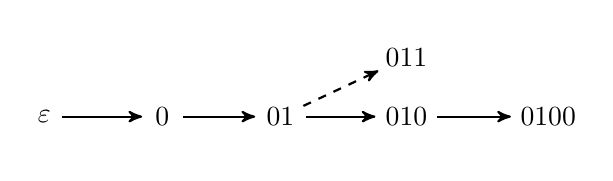
\begin{tikzpicture}[->,>=stealth',auto,thick, scale = 1.0,state/.style={circle,inner sep=2pt}]

    % The graph
	\node [state] at (0,0) (R) {$\varepsilon$};
	\node [state] at (1.5,0) (0) {$0$};
	\node [state] at (3,0) (01) {$01$};
	\node [state] at (4.6,0) (010) {$010$};
	\node [state] at (6.4,0) (0100) {$0100$};
	
	\node [state] at (4.6,0.75) (011) {$011$};					
	
	% Graph edges
	\path[->]
	(R) edge (0)
	(0) edge (01)
	(01) edge (010)
	(010) edge (0100)	
	;  	
	
	\path[->,dashed]
	(01) edge (011)
	;


\end{tikzpicture} 
\end{center}
\caption{If playing $\forkm{2}_1$, player 1 will try to fork after losing two consecutive blocks at position 0100. Should she manage to make the dashed branch into a blockchain, both her and player 1 continue to mine on this branch using $\df$.}
\label{fig-fork_m}
\end{figure}

When computing the utility of $\forkm{m}$ starting in some state $q_0$, we take into account that player 1 is only interested whether her utility will increase in the case she decides to fork. That is, since the blocks before her fork will always have the same constant contribution to her reward in either branch, we will not count them in the utility. With this in mind, the utility of $\forkm{m}$ starting in the state $q_0$ in which 0 has the ultimate $m$ blocks in the (up to now unique) blockchain is given as follows.

\begin{myprop}\label{prop-fork_m}
	Let $h$ be the hash power of player 1. Then
	\begin{eqnarray*}
		u_1(\mfork|q_0) =K_{1}Cat(\beta^2h(1-h))^{m+1}+K_{2}Cat(\alpha\beta^2h(1-h))^{m+1}
	\end{eqnarray*}
	where Cat is as in Proposition \ref{prop:utility_gen_fork}, and $K_1,K_2$ are constants depending on $\alpha,\beta,h$ and $m$.
\end{myprop}

As before, Catalan numbers help us account for all states where 1 wins the fork. Of course, now player 1 is starting with a handicap of $m$ steps, so the winning states for 1 will be characterized by staircase walks that stay inside the trapezoid $\{(0,0),(m,0),(m+n,n),(0,n)\}$, for some number $n$. The proof of this proposition is given in Appendix \ref{appendix-fork_m}.

\paragraph{When to fork?} Having the utilities of the two forking strategies, we can now compare them to that of the default strategy in order to answer whether 1 should fork or not. Analysing the curves defined by the game parameters ($\alpha,\beta$ and $h$ for $\fg$, and additionally $m$ for $\forkm{m}$), it can be seen that when $h>50\%$, and $\alpha>\beta$, then it is always convenient for 1 to fork, based on the utility resulting from either $\fg$ or (irrespective of $m$) $\forkm{m}$. This confirms the intuition that the player with the majority of hash power can sway the game in her favour, but we can also see that there are several cases when it is convenient to fork even with much lower hash power. This happens in cases when $\alpha$ is significantly bigger than $\beta$, which can be explained by the fact that ???

%(probably say this is a very interesting open question in the literature). 
%
%In order to understand when forking could be a good strategy, let us consider again the two player game in which player $p$ has just mined a block in the blockchain. 
%Now, if player $(1-p)$ wins the next block, player $p$ faces two different options. She could continue mining on the blockchain, playing according to $\df$, or she 
%could fork, mining instead upon her previously won block. Which strategy is better? To answer this question, we need to calculate the utility in both cases. For 
%simplicity, and without loss of generality (due to Lemma [?]), we will focus on this question when the game is just starting, in the genesis block, and we will assume that 
%player $p$ resumes the default strategy (mining upon the blockchain) as soon as she wins the fork. 
%
%More precisely, we will calculate the utility of the combined strategy $(\df_{1-p},\fg_p)$, where $\fg_p$ is the \textbf{Fork on the genesis} 
%strategy, defined as follows for a state $q \in \bQ$:
%%\begin{eqnarray*}
%%\fg_p(q) & = &
%%\begin{cases}
%%\mine(p,\varepsilon,q) & \text{if } p \not\in q\\
%%\mine(p,\bchain(q),q) &  \text{if } \bchain(q) \text{ is defined and } p \preceq \bchain(q)\\
%%\mine(p,b,q) &  \text{if } \bchain(q) \text{ is defined},\  p \in q,\ p \not\preceq \bchain(q)
%%\text{ and}\\
%%&  \hspace{50pt} {\displaystyle b = \max_{\preceq} \, \{ b' \in q \mid \longest(q,p) \preceq b'\}}\\
%%\mine(p,\longest(q,p),q) &  \text{if } \bchain(q) \text{ is not defined},\ p \in q \text{ and}\\
%%& \hspace{50pt} p \not\preceq \longest(q,1-p)\\
%%\mine(p,\longest(q,p),q) &  \text{if } \bchain(q) \text{ is not defined},\ p \preceq \longest(q,1-p) \text{ and}\\
%%& \hspace{50pt} r_p(\longest(q,p)) \geq r_p(\longest(q,1-p))\\
%%\mine(p,\longest(q,1-p),q) &  \text{if } \bchain(q) \text{ is not defined},\  p \preceq \longest(q,1-p) \text{ and}\\
%%& \hspace{50pt} r_p(\longest(q,p)) < r_p(\longest(q,1-p))
%%\end{cases}
%%\end{eqnarray*}
%\begin{eqnarray*}
%\fg_p(q) & = &
%\begin{cases}
%\mine(p,\varepsilon,q) & \text{if } p \not\in q\\
%\df_p(q) & \text{if } \bchain(q) \text{ is defined and } p \preceq \bchain(q) \text{ or}\\
%& \hspace{70pt} \bchain(q) \text{ is not defined and } p \preceq \longest(q,1-p)\\
%\mine(p,b,q) &  \text{otherwise, where } {\displaystyle b = \max_{\preceq} \, \{ b' \in q \mid \longest(q,p) \preceq b'\}}
%\end{cases}
%\end{eqnarray*}
%Notice that in this definition, the set $\{ b' \in q \mid \longest(q,p) \preceq b'\}$ has a maximum element under the partial order $\preceq$ as all the elements in this set are of the form $\longest(q,p) \cdot (1-p)^\ell$ with $\ell \geq 0$.
%
%(show how to compute the utility, put graphics, compare. 
%
%\subsection{More complicated cases}
%
%Speak of $m$-fork as a refinement of the previous strateegy, put give-up time if we have it as well. Graphics, compare, etc. 
%
%\subsection{Stationary equilibrium}
%
%Need to fill this up! 

	
	%%!TEX root = focs.tex

\section{OLD SECTION (still need to move a lot of material): Full Disclosure Scenario and Two Players}
\label{sec-fd&2p}

We can use Proposition \ref{prop-length-greedy} to simplify the definition of greedy actions. More specifically, assume that $p \in \{0,1\}$ and $q \in \bQ$, and from now let $\longest(q,p)$ be a string instead of a singleton set. Then the conditions in Definition \ref{def-greedy} for a valid action $\mine(p,b,q)$ can be restated as follows:
\begin{itemize}
\item If $\bchain(q)$ is defined, then $|\longest(q,p)| \leq |b|  \leq \bchain(q)$. In particular, if $\owner(\bchain(q)) = p$, then $b = \bchain(q)$ (and, thus, $p$ attempts to mine in the last block in the blockchain as this block is hers).

\item If $\bchain(q)$ is not defined, then $b = \longest(q,0)$  or $b = \longest(q,1)$. 
\end{itemize}
Then for the mining game, we consider the following strategies:
\begin{itemize}
\item {\bf The default strategy.}  The first strategy we describe will be called $\df$, and it will reflect the desired behaviour of the miners participating in the Bitcoin network. Intuitively, in a state $q$, a player following this strategy will try to mine upon the final block that appears in the blockchain of $q$. If the blockchain in state $q$ does not exist, meaning that there are two longest paths from the genesis block, then the player will mine on the final block of one of these paths according to her rewards in them (she will choose the one that maximizes her reward). Given a player $p \in \{0,1\}$, we call this strategy $\df_p$, and we define it as follows for a state $q \in \bQ$:
\begin{eqnarray*}
\df_p(q) & = &
\begin{cases}
\mine(p,\bchain(q),q) & \text{if } \bchain(q) \text{ is defined}\\
\mine(p,\longest(q,p),q) & \text{if } \bchain(q) \text{ is not defined and} \\
& \hspace{40pt} r_p(\longest(q,p)) \geq r_p(\longest(q,1-p))\\
\mine(p,\longest(q,1-p),q) & \text{if } \bchain(q) \text{ is not defined and}\\
& \hspace{40pt} r_p(\longest(q,p)) < r_p(\longest(q,1-p))
\end{cases}
\end{eqnarray*}

\item {\bf Fork on the genesis.} Given a player $p \in \bP$, we call this strategy $\fg_p$, and we define it as follows for a state $q \in \bQ$:
%\begin{eqnarray*}
%\fg_p(q) & = &
%\begin{cases}
%\mine(p,\varepsilon,q) & \text{if } p \not\in q\\
%\mine(p,\bchain(q),q) &  \text{if } \bchain(q) \text{ is defined and } p \preceq \bchain(q)\\
%\mine(p,b,q) &  \text{if } \bchain(q) \text{ is defined},\  p \in q,\ p \not\preceq \bchain(q)
%\text{ and}\\
%&  \hspace{50pt} {\displaystyle b = \max_{\preceq} \, \{ b' \in q \mid \longest(q,p) \preceq b'\}}\\
%\mine(p,\longest(q,p),q) &  \text{if } \bchain(q) \text{ is not defined},\ p \in q \text{ and}\\
%& \hspace{50pt} p \not\preceq \longest(q,1-p)\\
%\mine(p,\longest(q,p),q) &  \text{if } \bchain(q) \text{ is not defined},\ p \preceq \longest(q,1-p) \text{ and}\\
%& \hspace{50pt} r_p(\longest(q,p)) \geq r_p(\longest(q,1-p))\\
%\mine(p,\longest(q,1-p),q) &  \text{if } \bchain(q) \text{ is not defined},\  p \preceq \longest(q,1-p) \text{ and}\\
%& \hspace{50pt} r_p(\longest(q,p)) < r_p(\longest(q,1-p))
%\end{cases}
%\end{eqnarray*}
\begin{eqnarray*}
\fg_p(q) & = &
\begin{cases}
\mine(p,\varepsilon,q) & \text{if } p \not\in q\\
\df_p(q) & \text{if } \bchain(q) \text{ is defined and } p \preceq \bchain(q) \text{ or}\\
& \hspace{70pt} \bchain(q) \text{ is not defined and } p \preceq \longest(q,1-p)\\
\mine(p,b,q) &  \text{otherwise, where } {\displaystyle b = \max_{\preceq} \, \{ b' \in q \mid \longest(q,p) \preceq b'\}}
\end{cases}
\end{eqnarray*}
Notice that in this definition, the set $\{ b' \in q \mid \longest(q,p) \preceq b'\}$ has a maximum element under the partial order $\preceq$ as all the elements in this set are of the form $\longest(q,p) \cdot (1-p)^\ell$ with $\ell \geq 0$.

%\item {\bf Fork on the $\ell$-th block of the blockchain.} Given a player $p \in \bP$, we call this strategy $\fork_{p,\ell}$, and we define it as follows for a state $q \in \bQ$:
%\begin{eqnarray*}
%\fork_p(q) & = &
%\begin{cases}
%\mine(p,\varepsilon,q) & \text{if } p \not\in q\\
%\mine(p,\bchain(q),q) &  \text{if } \bchain(q) \text{ is defined and } p \preceq \bchain(q)\\
%\mine(p,\longest(q,p),q) &  \text{if } \bchain(q) \text{ is defined},\  p \in q \text{ and } p \not\preceq \bchain(q)\\
%\mine(p,\longest(q,p),q) &  \text{if } \bchain(q) \text{ is not defined},\ p \in q \text{ and}\\
%& \hspace{50pt} p \not\preceq \longest(q,1-p)\\
%\mine(p,\longest(q,p),q) &  \text{if } \bchain(q) \text{ is not defined},\ p \preceq \longest(q,1-p) \text{ and}\\
%& \hspace{50pt} r_p(\longest(q,p)) \geq r_p(\longest(q,1-p))\\
%\mine(p,\longest(q,1-p),q) &  \text{if } \bchain(q) \text{ is not defined},\  p \preceq \longest(q,1-p) \text{ and}\\
%& \hspace{50pt} r_p(\longest(q,p)) < r_p(\longest(q,1-p))
%\end{cases}
%\end{eqnarray*}

\item {\bf Fork on the genesis with give up time.} Given a player $p \in \bP$ and a natural number $k \geq 1$, we call this strategy $\fg_{p,k}$, and we define it as follows for a state $q \in \bQ$:
\begin{eqnarray*}
\fg_{p,k}(q) & = &
\begin{cases}
\mine(p,\longest(q,1-p),q) & \text{if } \length(q,1-p) - \length(q,p) > k\\
\fg_p(q) &   \text{otherwise}
\end{cases}
\end{eqnarray*}

\item {\bf Forking repeatedly.} Given a player $p \in \bP$, we call this strategy $\fr_{p}$, and we define it as $\mine(p, \longest(q,p), q)$ for every state $q \in \bQ$.

\item {\bf Forking repeatedly with give up time.} Given a player $p \in \bP$ and a natural number $k \geq 1$, we call this strategy $\fr_{p,k}$, and we define it as follows for a state $q \in \bQ$:
\begin{eqnarray*}
\fr_{p,k}(q) & = &
\begin{cases}
\mine(p,\longest(q,1-p),q) & \text{if } \length(q,1-p) - \length(q,p) > k\\
\mine(p,\longest(q,p),q) & \text{otherwise}
\end{cases}
\end{eqnarray*}


%\begin{eqnarray*}
%\fr_{p,k}(q) & = &
%\begin{cases}
%\mine(p,b,q) & \text{if } \length(q,1-p) - \length(q,p) > k, \text{ where}\\
%& \hspace{20pt} {\displaystyle b = \max_{\preceq}\, \{ b' \in q \mid b' \preceq \bchain(q) \text{ and } b' = \varepsilon \text{ or } 
%
%\owner(b') = p \text{ and } \length(q,1-p)
%\fg_p(q) &   \text{otherwise}
%\end{cases}
%\end{eqnarray*}
\end{itemize}




\paragraph{Longest blocks and optimal strategies.}
For a body of knowledge $q$ and a block $b \in q$, let us denote by $\subbody(q,b)$ the body of knowledge 
given by $\{u \mid b\cdot u$ is a block in $q\}$, that is, the subtree of $q$ rooted at $b$, but in which $b$ is renamed 
$\epsilon$ and all its descendants are renamed accordingly. 

%Furthermore, let us denote by $\meet(q,p)$ the greatest block in the set $\{b \in q \mid b$ is a prefix all nodes in $\longest(q)\}$, the greatest common block owned by $p$ that is a prefix of all 
%blocks in $\longest(q)$. 

The following Lemma tells us that an optimal strategy for player $p$ can only differentiate the portion of 
a body of knowledge that goes after $\meet(q,p)$: 

\begin{mylem}
Let $s = (s_1,s_2)$ be a $\beta$ discounted stationary equilibrium in an infinite mining game with two players. 
Then there is a $\beta$ discounted stationary equilibrium such that $u_p(s \mid q_0) = u_p(s' \mid q_0)$ for 
any player $p$ and for every pair $q$ and $q'$ of 
bodies of knowledge in which $\subbody(q,\meet(q,p)) = \subbody(q',\meet(q',p))$ we have that 
$s_p(q) = s_p(q')$. 
\end{mylem}

\begin{proof}
\end{proof}



%To this end, given a player $p \in \bP$ and a body of knowledge $q$,
%
%
% Let $q$ be a body of knowledge. 
%
%
%terminology. 
%
%
%given a body of knowledge, we assume that 


%For the mining game we will consider the following strategies:
%\begin{itemize}
%\item {\bf The default strategy.}  The first strategy we describe will be called $\df$, and it will reflect the desired behaviour of the miners participating in the Bitcoin network. Intuitively, in a state $q$, a player following this strategy will try to mine upon the final block that appears in the blockchain of $q$. If the blockchain in state $q$ does not exist, meaning that there are two longest paths from the genesis block, the player will mine on the final block of the path that contains the highest number of her blocks. We call this strategy \df, and we define it formally as follows:
%
%\begin{eqnarray*}
%\df_p(q) & = &
%\begin{cases}
%\mine(p,\last(\bchain(q)),q) & \text{if } \bchain(q) \text{ exists }\\
%\mine(p,\cho(q),q) & \text{if } \bchain(q) \text{ does not exist }
%\end{cases}
%\end{eqnarray*}
%
%%Here $last(\bchain(q))$ returns the last block in $\bchain(q)$, and $best(q)$ returns the last block of the path that is of maximal length in $q$, and on which the player $p$ has the highest number of blocks compared to all maximal paths in $q$. If there is more than one such path, $best(q)$ is the one that is smallest lexicographically. Intuitively, $best(q)$ is the block on which a benevolent player will mine upon when it is not clear what the blockchain is.
%
%\item {\bf Fork on the $k$th block from the end of the blockchain.} If we assume two players, one of them playing the default strategy, and the other will fork only once, this means that the fork will happen in some state where the blockchain is defined. This strategy says that the player that will fork, does this by mining on a block that is $k$ blocks away from $\last(\bchain(q))$. Following this, the player always mines on the last block of this chain. $k=\infty$ means fork on genesis. 
%
%\francisco{I think this needs to be rephrased. And maybe separate the case $k=\infty$ as a different strategy altogether, for two reasons: 1) it represents a Satoshi-gate, the motivation behind it is more than just stealing blocks, and 2) the case $k=\infty$ is way easier to compute (just Catalan numbers) and it is good to introduce the finite $k$ case (trapezoidal Dyck paths). }
%
%\item {\bf Fork on the $k$th block belonging to me counting from the end of the blockchain.} Similar to the previous strategy, but this time the player will mine on the $k$th block belonging to her, counting from $\last(\bchain(q))$. Following this, the player always mines on the last block of this chain. With $k=1$ the player are forking on her ultimate block in the blockchain, and with $k=\infty$ in the genesis.
%
%\item {\bf Give up time $g$.} This can be a parameter in any of the above strategies. Once forked, if the branch belonging to the non forking player is $g$ block ahead of the forking branch, the game continues on this branch with no more forks.
%\end{itemize}
%
%
%\francisco{Some results follow, only for the $\alpha$ discounted utility, without delay. Should we compute this for other utilities or rewards? Should we put the proof into the appendix?}
\subsection{Utility of default strategy}
In this section, players $\{1,2\}$ play according to the default strategy, defined in section \ref{sec-fd&2p}. For any state $q$ of the game, $\mathcal{T}(q)$ consists of a single branch and therefore \bchain$(q)$ is always defined. Moreover, given the behavior of players we can write $q$ uniquely as a binary sequence $w\in\{0,1\}^{\mid q\mid }$ encoding the chronological history of the game until $q$ is reached, where $1$ stands for ``player 1 appends a block'' and $0$ stands for ``player 2 appends a block''. In other words, there is a bijection $ \bQ \simeq\bchain(\bQ)\simeq \{0,1\}^\ast$. This encoding proves useful as we have
\begin{eqnarray*}
	r_p(w) &=&	c\cdot \sum_{j=1}^{\mid w\mid}w[j] \alpha^j  \\
	\pr^{\df}(w \mid \varepsilon) &=&	h^{H(w)}(1-h)^{|w|-H(w)}
\end{eqnarray*}
where $H(x)$ denotes the Hamming weight of integer $x$, defined as the amount of non-zero bits of $x$. We prove the following.


\begin{myprop*}
Let $h$ denote the hash power of player 1. Then 
$$u_1^n(\df\mid\varepsilon) = \frac{\alpha\beta^{n+2}+\alpha(1-\beta)(\alpha\beta)^{n+1}+\beta^{n+1}+(1-\alpha)}{(1-\alpha)(1-\beta)(1-\alpha\beta)}\cdot h c.$$
In particular,
$$u_1^\infty(\df\mid\varepsilon) = \frac{hc}{(1-\beta)(1-\alpha\beta)}.$$
\end{myprop*}
\begin{proof}

\begin{eqnarray*}
u_1^n(\df \mid \varepsilon) & = & \sum_{i=0}^{n}\beta^{i} \cdot  \bigg(\sum_{\substack{q \in \bQ \,: |q| = i}} r_1(q) \cdot 
\pr^{\df}(q \mid \varepsilon)\bigg)\\
							& = & c\cdot \sum_{i=0}^{n}\beta^{i} \cdot\bigg(\sum_{w\in\{0,1\}^i}  \bigg( \sum_{j=1}^{i}w[j] \alpha^j \bigg)\cdot 
\pr^{\df}(w \mid \varepsilon)\bigg)\\
							& = & c\cdot \sum_{i=0}^{n}\beta^{i}\sum_{j=1}^{i} \alpha^j \cdot\bigg(\sum_{w\in\{0,1\}^i}   w[j]\cdot 
\pr^{\df}(w \mid \varepsilon)\bigg)\\
							& = & c\cdot \sum_{i=0}^{n}\beta^{i}\sum_{j=1}^{i} \alpha^j \expected(w[j]) = ch\cdot \sum_{i=0}^{n}\beta^{i}\sum_{j=1}^{i} \alpha^j 
\end{eqnarray*}
yielding the result, where we used the facts that ownership of different blocks are independent Bernoulli trials with probability of success $h$ and $\pr(\{0,1\}^i)=1$ for all $i$.
\end{proof}

\subsection{Utility of the genesis fork}
\label{sec-genfork}
Suppose player 2 follows the default strategy, and player 1 attempts to fork once at the genesis block $\varepsilon$, as described in section \ref{sec-fd&2p} (case $k=\infty$).
\francisco{TBH I dislike the previous notation} As a result of this behavior, for any state of the game $\cT(q)$ consists in a rooted tree in $\varepsilon$ with at most two branches. We can naturally refer to these as the original branch (the one player 2 is mining until the forks succeeds) and the new branch. Note that in this scenario we also have a bijection $\bQ\simeq \{0,1\}^\ast$, since the chronological history of mined blocks allows to uniquely determine any state of the game. Hence, we encode any state $q\in Q$ as a binary string with the instructions 0 (player 2 appends a block) and 1 (player 1 appends a block). For any binary string $x$, let $\Delta(x)$ denote the amount of zeros minus the amount of ones in $x$.

\begin{mydef}
 A Dyck draw is a binary string $d$ such that $\Delta(d)=0$ and every initial substring $d'$ of $d$ verifies $\Delta(d')\leq 0$. We denote by $\Dyck_{2n}$ the set of Dyck draws of length $2n$ and $\Dyck^\ast$ the set of all Dyck draws.
\end{mydef}

Denote by $\bQ'\subsetneq \bQ$ the states in which player 1 has a positive reward. We can write $\bQ'$ as a disjoint union as follows. First note that before the new branch becomes $\bchain(q)$ for some state $q$ in the game, player 1 receives no reward, (\ie $q\notin \bQ'$). On the other hand, if $\bchain(q)$ includes the new branch for a state $q\in Q$, then $q$ contains an initial string of the form $d1$ where $d\in \Dyck^\ast$. Therefore,
$$\bQ'\simeq \bigcup_{k=0}^\infty \{d1w,d\in \Dyck^{2k},w\in \{0,1\}^\ast\}$$

With this, we can prove the following.
\begin{myprop*}
Suppose player 1 plays with the genesis fork strategy and player 2 follows the default strategy. Let $h$ be the hash power of player 1. Then
\begin{eqnarray*}
	u_1^n(\gf \mid \varepsilon) & = & \sum_{i=0}^{n} \bigg( \sum_{\substack{2k+1+l=i\\k\geq 0,l\geq 0}} C_k\cdot \beta^{i} \cdot S_{l,k}(\alpha,h)\cdot h^{k+1}(1-h)^{k} \bigg)
\end{eqnarray*}
where $C_k={2k\choose k}/(k+1)$ is the $n$-th Catalan number and $S_{l,k}(\alpha,h)=\frac{1}{1-\alpha}(1+\alpha^{k+1}(h-1)-h\alpha^{l+k+1})$. In particular,
\begin{eqnarray*}
	u_1^\infty(\gf \mid \varepsilon) & = & K_1 c(\alpha\beta^2h(1-h))+K_2 c(\beta^2h(1-h))
\end{eqnarray*}
for some constants $K_1,K_2$ where $c:x\mapsto \frac{1-\sqrt{1-4x}}{2x}$ is the generating function of Catalan numbers.

\end{myprop*}
\begin{proof} Every state of positive reward $q\in\bQ'$ is of the form $d1w$ for a Dyck draw $d$ and $w\in \{0,1\}^\ast$. Denote $w[i]$ the $i$-th bit of $w$, with $i=1,\dots,|w|$. Note that

\begin{eqnarray*}
r_1(d1w) &=& c\cdot \bigg(\bigg(\sum_{i=0}^{|d|-1}\alpha^i \bigg)+\alpha^{|d|}+\alpha^{|d|+1}\bigg(\sum_{i=0}^{|w|-1}\alpha^i w[i]\bigg)\bigg),\\
\pr^{\gf}(d1w|\varepsilon) &=& h^{|d|/2+1+H(w)}(1-h)^{|d|/2+|w|-H(w)}.
\end{eqnarray*} 
With this we can compute 
\begin{eqnarray*}
	u_1^n(\gf \mid \varepsilon) & = & \sum_{i=0}^{n}\beta^{i} \cdot  \bigg(\sum_{\substack{q \in \bQ' \,: |q| = i}} r_1(q) \cdot 
	\pr^{\gf}(q \mid \varepsilon)\bigg)\\
								& = & \sum_{i=0}^{n}\beta^{i} \cdot  \bigg(\sum_{2k+1+l=i}\sum_{\substack{d\in \Dyck_{2k}\\w\in\{0,1\}^l}} r_1(d1w) \cdot 
	\pr^{\gf}(d1w \mid \varepsilon)\bigg).
\end{eqnarray*}
First note that in the inner sum, the expressions $r(d1w)$ and $\pr^{\gf}(d1w|\varepsilon)$ depend only in $k,l$. Define
$$S_{k,l}(\alpha,h)=\sum_{w\in\{0,1\}^l}r(d1w)\cdot \pr^{\gf}(w|d1)$$
and compute $S_{k,l}(\alpha,h)$ using the facts $\pr^{\gf}(\{0,1\}^l|d1)=1$ and $\expected(w[i])=h$ for every $i=1,\dots,l$, obtaining the claimed expression. We have
\begin{eqnarray*}
u_1^n(\gf \mid \varepsilon) & = & \sum_{i=0}^{n}\beta^{i} \cdot  \bigg(\sum_{2k+1+l=i} \#(\Dyck_{2k})\cdot S_{l,k}(\alpha,h)\cdot h^{k+1}(1-h)^{k}\bigg).
\end{eqnarray*}
It is widely known that $\Dyck_{2k}=C_k$, where $C_k$ is the $k$-th Catalan number, yielding the result. \francisco{TODO: Exact constants, $n=\infty$ case, references to Catalan (Stanley's book)}
\end{proof}


\subsection{Utility of the $m$-fork strategy}

\francisco{I need a notation for this strategy. For the time being I'll use $\mfork$}

In the same strategy framework as section \ref{sec-genfork}, we now suppose that player 1 attempts to fork once, but instead of mining upon the genesis block, she only goes back $m$ blocks on an already defined blockchain of arbitrary length. In other words, let $c$ be the current blockchain of length $|c|\geq m$, and let $b_{-m}$ the block at position $|c|-m$. We also suppose that $\owner(b_{-m+i})=2$ for all $i=1,\dots,m$. Also, for the sake of simplicity and without loss of generality, in the computation of utility we don't count any reward given at blocks before $b_{-m}$ (these rewards acting as additive constants). Let us define the following.


\begin{mydef}
	A Dyck draw of disadvantage $m\in\NN$ is a binary string $d\in\{0,1\}^\ast$ such that $\Delta(d)+m=0$ and every initial substring $d'$ of $d$ verifies $\Delta(d')+m\leq 0$. We denote by $\Dyck_{2n,m}$ the set of Dyck draws of disadvantage $m$ of length $2n+m$ and $\Dyck^\ast_{m}$ the set of all Dyck draws of disadvantage $m$.
\end{mydef}

\begin{myprop*}
	\label{prop-trapezoidcardinality}
	Let $(n,m)\in \NN^2$, then 
	$$\#\Dyck_{2n,m}=\frac{m+1}{m+n+1}{m+2n\choose m+n}.$$
\end{myprop*}
\begin{proof}
Consider the north-east unitary steps $(\uparrow,\rightarrow)=((1,0),(0,1))$ in $\ZZ^2$, and let $d\in \Dyck_{2n,m}$. The bits in $d$ define a path from $(0,0)$ to $(n+m,n)$ where $0:\uparrow$ and $1:\rightarrow$. Because $d$ is a $m$-disadvantaged Dyck draw, this path stays inside the trapezoid $\{(0,0),(m,0),(m+n,n),(0,n)\}$. We count all such paths in appendix \ref{appendix-trapezoid}, obtaining the claimed expression.
\end{proof}
Now, as before note that every state of positive reward for player 1 is a state that successfully orphaned blocks from the original chain. The binary encoding can be written as $d1w$, where $d$ is a Dyck draw with disadvantage $m$ and $w\in\{0,1\}^\ast$ represent default playing by both players after the fork succeeds. 

\begin{myprop*}
If players 1 and 2 follow \mfork and \df strategies respectively, and if $h\in [0,1]$ is the hash power of player 1, then

\begin{eqnarray*}
	u_1^n(\mfork \mid \varepsilon) & = & \sum_{i=0}^{n}\beta^{i} \cdot  \bigg(\sum_{2k+1+l+m=i} \frac{m+1}{m+k+1}{m+2k\choose m+k} \cdot S'_{l,k,m}(\alpha,h)\cdot h^{k+1+m}(1-h)^{k}\bigg).
\end{eqnarray*}
In particular,
\begin{eqnarray*}
	u_1^\infty(\mfork \mid \varepsilon) & = & K_1 c(\alpha\beta^2h(1-h))^{m+1}+K_2 c(\beta^2h(1-h))^{m+1}
\end{eqnarray*}
for some constants $K_1,K_2$.

\end{myprop*}
\begin{proof}
	Let $\bQ'\subsetneq \bQ$ the set of states of positive reward for player 1. We have, as before, the disjoint union
	$$\bQ' = \bigcup_{k=0}^\infty \{d1w,\; d\in\Dyck_{2k,m}, w\in\{0,1\}^\ast\}.$$
	The reward and probability of a state $q=d1w\in \bQ'$ with $d\in\Dyck_{2k,m}$ and $w\in\{0,1\}^l$ are given by
\begin{eqnarray*}
	r_1(d1w) &=& c\cdot \bigg(\bigg(\sum_{i=-m}^{k-1}\alpha^i \bigg)+\alpha^{k}+\alpha^{k}\bigg(\sum_{i=1}^{l}\alpha^i w[i]\bigg)\bigg),\\
	\pr^{\gf}(d1w|\varepsilon) &=& h^{k+m+1+H(w)}(1-h)^{k+l-H(w)}.
\end{eqnarray*} 
We now compute
\begin{eqnarray*}
	u_1^n(\mfork \mid \varepsilon) & = & \sum_{i=0}^{n}\beta^{i} \cdot  \bigg(\sum_{\substack{q \in \bQ' \,: |q| = i}} r_1(q) \cdot 
	\pr^{\gf}(q \mid \varepsilon)\bigg)\\
								   & = & \sum_{i=0}^{n}\beta^{i} \cdot  \bigg(\sum_{2k+1+l+m=i}\sum_{\substack{d\in \Dyck_{2k,m}\\w\in\{0,1\}^l}} r_1(d1w) \cdot 
	\pr^{\gf}(d1w \mid \varepsilon)\bigg)\\
								   & = & \sum_{i=0}^{n}\beta^{i} \cdot  \bigg(\sum_{2k+1+l+m=i} \#(\Dyck_{2k,m})\cdot S'_{l,k,m}(\alpha,h)\cdot h^{k+1+m}(1-h)^{k}\bigg).
\end{eqnarray*}
where
$$S'_{l,k,m}=\sum_{w\in\{0,1\}^l}r(d1w)\pr^\mfork(w|d1)$$
can be computed as in section $\ref{sec-genfork}$. Finally, use proposition \ref{prop-trapezoidcardinality} to establish the result.
\end{proof}


	
	\bibliographystyle{plain}
	\bibliography{bibliography}
	\appendix
	
	%%!TEX root = focs.tex

\section{Proofs and definitions for Section \ref{sec-const_rew}}
\label{app-const}

DEFINE STRATEGIES HERE??

OR IN AN APPENDIX BEFORE THIS ONE?

\paragraph{Longest paths in greedy strategies.}

\begin{mylem}\label{lem-length-greedy}
Let $\bs$ be a greedy strategy. Then for every $q \in \bQ$ such that $\pr^{\bs}(q \mid \varepsilon) > 0$, the following conditions hold:
\begin{enumerate}
\item For every $p \in \{0,1\}$: $|\longest(q,p)| = 1$ 

\item $1 \leq |\longest(q)| \leq 2$

\item If $|\longest(q)| = 2$, then $\longest(q) = \longest(q,0) \cup \longest(q,1)$
\end{enumerate}
\end{mylem}

\begin{proof}
Let $S = \{ q \in \bQ \mid \pr^{\bs}(q \mid \varepsilon) > 0 \}$. Then we have that $S$ is the smallest subset of $\bQ$ satisfying the following conditions:
\begin{itemize}
\item $\{\varepsilon\} \in S$.

\item If $p \in \{0,1\}$, $b \in \bB$, $q \in S$ and $\mine(p,b,q)$ is a greedy action, then $q \cup \{ b \cdot p\} \in S$.
\end{itemize}
Hence, we have an inductive definition of $S$, and we can prove the proposition by induction on the structure of this set of states. If $q = \{ \varepsilon \}$, then we have that $\longest(q) = \longest(q,1) = \longest(q,2) = \{ \varepsilon \}$ and, thus, we have that  the three conditions in the proposition hold since $|\longest(q)| = |\longest(q,0)| = |\longest(q,1)| = 1$. Assume that the property holds for $q \in S$, and assume that $p \in \{0,1\}$, $b \in \bB$ and $\mine(p,b,q)$ is a greedy action. Then we need to prove that the conditions in the proposition hold for $q ' = q \cup \{b \cdot p \}$, for which we consider the following cases.
\begin{itemize}
\item Assume that $\longest(q,0) = \{b_0\}$,  $\longest(q, 1) = \{b_1\}$ and $\longest(q) = \{b_0,b_1\}$, and without loss of generality assume that $p = 0$. Given that $|b_0| = |b_1|$ and $\mine(p,b,q)$ is a greedy action, we have that either $b = b_0$ or $b = b_1$. If $b = b_0$, then it holds $b_0 \cdot 0 \in q'$, from which we conclude that the three conditions of the proposition hold since $\longest(q',0) = \{b_0 \cdot 0\}$, $\longest(q',1) = \{b_1\}$ and $\longest(q') = \{b_0 \cdot 0\}$.  If $b = b_1$, then it holds $b_1 \cdot 0 \in q'$, from which we conclude that the three conditions of the proposition hold since $\longest(q',0) = \{b_1 \cdot 0\}$, $\longest(q',1) = \{b_1\}$ and $\longest(q') = \{b_1 \cdot 0\}$.

\item Assume that $\longest(q,0) = \{b_0\}$,  $\longest(q, 1) = \{b_1\}$ and $\longest(q) = \{b_0\}$, so that $|b_1| < |b_0|$. Notice that if $p =0$, then we have that $b=b_0$ since $\mine(p,b,q)$ is a greedy action. Hence, it holds $b_0 \cdot 0 \in q'$, from which we conclude that the three conditions of the proposition hold since $\longest(q',0) = \{b_0 \cdot 0\}$, $\longest(q',1) = \{b_1\}$ and $\longest(q') = \{b_0 \cdot 0\}$. Therefore, assume that $p = 1$, from which we have that  $|b_1| \leq |b|$ and $|b| \leq |b_0|$, since $\mine(p,b,q)$ is a greedy action and $\longest(q) = \{b_0\}$. Thus, given that $b \cdot 1 \in q'$, we conclude that $\longest(q',0) = \{b_0\}$ and $\longest(q',1) = \{b \cdot 1\}$. 
Moreover, if $|b \cdot 1| < |b_0|$, then it holds that $\longest(q') = \{b_0\}$ and the three conditions of the proposition are satisfied. If $|b \cdot 1| = |b_0|$, then we have that $\longest(q') = \{b_0, b \cdot 1\}$, from which we conclude that the three conditions of the proposition are satisfied since $|\longest(q')| = 2$ and $\longest(q') = \longest(q',0) \cup \longest(q',1)$. Finally, if $|b \cdot 1| > |b_0|$ (that is, if $b = b_0$), then $\longest(q') = \{b \cdot 1\}$ and again the three conditions of the proposition are satisfied.

\item Assume that $\longest(q,0) = \{b_0\}$,  $\longest(q, 1) = \{b_1\}$ and $\longest(q) = \{b_1\}$. This case is analogous to the previous case, which concludes the proof of the proposition.
\end{itemize}
\end{proof}


\paragraph{Longest blocks and optimal strategies.}
For a state $q$ and a block $b \in q$, let us denote by $\subbody(q,b)$ the state
given by $\{u \mid b\cdot u$ is a block in $q\}$, that is, the subtree of $q$ rooted at $b$, but in which $b$ is renamed 
$\epsilon$ and all its descendants are renamed accordingly. 

%Furthermore, let us denote by $\meet(q,p)$ the greatest block in the set $\{b \in q \mid b$ is a prefix all nodes in $\longest(q)\}$, the greatest common block owned by $p$ that is a prefix of all 
%blocks in $\longest(q)$. 

The following Lemma tells us that an optimal strategy for player $p$ can only differentiate the portion of 
a state that goes after $\meet(q,p)$: 

\begin{mylem}\label{lem-optimal}
Let $s = (s_1,s_2)$ be a $\beta$ discounted stationary equilibrium in an infinite mining game with two players. 
Then there is a $\beta$ discounted stationary equilibrium such that $u_p(s \mid q_0) = u_p(s' \mid q_0)$ for 
any player $p$ and for every pair $q$ and $q'$ of 
bodies of knowledge in which $\subbody(q,\meet(q,p)) = \subbody(q',\meet(q',p))$ we have that 
$s_p(q) = s_p(q')$. 
\end{mylem}

\begin{proof}
\end{proof}
	
\section{Proofs and Intermediate Results}
\subsection{Convergence of the utility function}
\label{sec-conver}

To ensure that the utility function $u_p(\bs \mid q_0)$ is well defined, we impose the restriction that for every payoff function $\bR = (r_0, \ldots, r_{m-1})$, there exists a polynomial $P$ such that $|r_p(q)| \leq P(|q|)$ for every player $p \in \bP$ and state $q \in \bQ$. In this section, we prove that this is indeed a sufficient condition for $u_p(\bs \mid q_0)$ to be a real number, for which we first need a technical lemma. 

\begin{mylem}\label{lem-prop-k}
Let $q_0 \in \bQ$ and $\bs$ be a combined strategy. Then for every $k \geq 0$, it holds that
\begin{eqnarray*}
\sum_{\substack{q \in \bQ \,: \\ q_0 \subseteq q \text{ {\rm and} } |q| - |q_0| = k}} \pr^{\bs}(q \mid q_0) & = & 1.
\end{eqnarray*}
\end{mylem}

\begin{proof}
We prove the lemma by induction on $k$. For $k=0$ the property trivially holds since $\pr^{\bs}(q_0 \mid q_0) = 1$. Thus, assuming that the property holds for $k$, we need to prove that it holds for $k+1$. We have that:
\begin{align*}
&\sum_{\substack{q \in \bQ \,: \\ q_0 \subseteq q \text{ {\rm and} } |q| - |q_0| = k+1}} \pr^{\bs}(q \mid q_0) \ =\\
&\hspace{30pt}\sum_{\substack{q \in \bQ \,: \\ q_0 \subseteq q \text{ {\rm and} } |q| - |q_0| = k+1}} 
\bigg(\sum_{\substack{q' \in \bQ \,: \\ q_0 \subseteq q' \text{ {\rm and} } |q'| - |q_0| = k}} \pr^{\bs}(q' \mid q_0) \cdot \pr(q',\bs(q'),q)\bigg) \ = \\
&\hspace{30pt}\sum_{\substack{q' \in \bQ \,: \\ q_0 \subseteq q' \text{ {\rm and} } |q'| - |q_0| = k}}
\bigg(\sum_{\substack{q \in \bQ \,: \\ q_0 \subseteq q \text{ {\rm and} } |q| - |q_0| = k+1}} 
 \pr^{\bs}(q' \mid q_0) \cdot \pr(q',\bs(q'),q)\bigg) \ =\\
 &\hspace{30pt}\sum_{\substack{q' \in \bQ \,: \\ q_0 \subseteq q' \text{ {\rm and} } |q'| - |q_0| = k}}
\pr^{\bs}(q' \mid q_0) \cdot \bigg(\sum_{\substack{q \in \bQ \,: \\ q_0 \subseteq q \text{ {\rm and} } |q| - |q_0| = k+1}} 
  \pr(q',\bs(q'),q)\bigg) \ =\\
&\hspace{30pt}\sum_{\substack{q' \in \bQ \,: \\ q_0 \subseteq q' \text{ {\rm and} } |q'| - |q_0| = k}}
\pr^{\bs}(q' \mid q_0) \cdot \bigg(\sum_{\substack{q \in \bQ \,: \\ q_0 \subseteq q,\ |q| - |q_0| = k+1,\ \bs(q') = (a_0, \ldots, a_{m-1}) \text{ {\rm and}}\\
\text{{\rm there exists }} p \in \{0, \ldots, m-1\} \text{ {\rm such that} } q = a_p(q')}}
  \pr(q',\bs(q'),q)\bigg) \ =\\
  &\hspace{30pt}\sum_{\substack{q' \in \bQ \,: \\ q_0 \subseteq q' \text{ {\rm and} } |q'| - |q_0| = k}}
\pr^{\bs}(q' \mid q_0) \cdot \bigg(\sum_{\substack{p \in \{0, \ldots, m-1\} \, : \\ \bs(q) = (a_0, \ldots, a_{m-1})}} \pr(q',\bs(q'),a_p(q'))\bigg) \ =\\
&\hspace{30pt}\sum_{\substack{q' \in \bQ \,: \\ q_0 \subseteq q' \text{ {\rm and} } |q'| - |q_0| = k}}
\pr^{\bs}(q' \mid q_0).
\end{align*}
Hence, given that
\begin{eqnarray*}
\sum_{\substack{q' \in \bQ \,: \\ q_0 \subseteq q' \text{ {\rm and} } |q'| - |q_0| = k}}
\pr^{\bs}(q' \mid q_0) & = & 1
\end{eqnarray*}
by induction hypothesis, we conclude that
\begin{eqnarray*}
\sum_{\substack{q \in \bQ \,: \\ q_0 \subseteq q \text{ {\rm and} } |q| - |q_0| = k+1}}
\pr^{\bs}(q \mid q_0) & = & 1.
\end{eqnarray*}
\end{proof}

\begin{myprop}\label{prop-conv}
Let $p \in \{0, \ldots, m-1\}$, $q_0 \in \bQ$ and $\bs$ be a combined strategy. If there exist a polynomial $P$ such that $|r_p(q)| \leq P(|q|)$ for every $q \in \bQ$, then $u_p(\bs \mid q_0)$ is a real number.
\end{myprop}

\begin{proof}
Notice that if $P$ is a zero polynomial, then the property trivially holds. Thus, we assume that $P$ is a nonzero polynomial. 
Then we have that:
\begin{eqnarray}
\notag
u_p(\bs \mid q_0) & =  & \sum_{q \in \bQ \,:\, q_0 \subseteq q} \beta^{|q|-|q_0|} \cdot  r_p(q) \cdot \pr^{\bs}(q \mid q_0)\\
\notag
& = & \sum_{n=0}^\infty \bigg(\sum_{\substack{q \in \bQ \,: \\ q_0 \subseteq q \text{ {\rm and} } |q| - |q_0| = n}} \beta^{|q|-|q_0|} \cdot  r_p(q) \cdot \pr^{\bs}(q \mid q_0)\bigg)\\
\label{eq-gen-form}
& = & \sum_{n=0}^\infty \beta^n \cdot \bigg(\sum_{\substack{q \in \bQ \,: \\ q_0 \subseteq q \text{ {\rm and} } |q| - |q_0| = n}} r_p(q) \cdot \pr^{\bs}(q \mid q_0)\bigg).
\end{eqnarray}
Let $f : \mathbb{N} \to \mathbb{R}$ be a function defined as:
\begin{eqnarray*}
f(n) & = & \sum_{\substack{q \in \bQ \,: \\ q_0 \subseteq q \text{ {\rm and} } |q| - |q_0| = n}} r_p(q) \cdot \pr^{\bs}(q \mid q_0).
\end{eqnarray*}
Notice that this function is well-defined as there exists a finite number of states $q \in \bQ$ such that $|q| - |q_0| = n$. Then by equation \eqref{eq-gen-form}, we have that:
\begin{eqnarray*}
u_p(\bs \mid q_0) & = & \sum_{n=0}^\infty \beta^n \cdot f(n).
\end{eqnarray*}
Therefore, to show that $u_p(\bs \mid q_0)$ is a real number, we need to show that the series $ \sum_{n=0}^\infty \beta^n \cdot f(n)$ converges, for which we prove that the series $ \sum_{n=0}^\infty |\beta^n \cdot f(n)|$ converges (that is, we show that $ \sum_{n=0}^\infty \beta^n \cdot f(n)$ converges absolutely, which is known to imply that this series is convergent). By definition of function $f$, we have that:
\begin{eqnarray}
\notag
|f(n)| & = & \bigg| \sum_{\substack{q \in \bQ \,: \\ q_0 \subseteq q \text{ {\rm and} } |q| - |q_0| = n}} r_p(q) \cdot \pr^{\bs}(q \mid q_0) \bigg|\\
\notag
& \leq & \sum_{\substack{q \in \bQ \,: \\ q_0 \subseteq q \text{ {\rm and} } |q| - |q_0| = n}} |r_p(q)| \cdot \pr^{\bs}(q \mid q_0)\\
\notag
& \leq & \sum_{\substack{q \in \bQ \,: \\ q_0 \subseteq q \text{ {\rm and} } |q| - |q_0| = n}} P(n) \cdot \pr^{\bs}(q \mid q_0)\\
\label{eq-f-abs}
& = & P(n) \cdot \bigg(\sum_{\substack{q \in \bQ \,: \\ q_0 \subseteq q \text{ {\rm and} } |q| - |q_0| = n}} \pr^{\bs}(q \mid q_0)\bigg).
\end{eqnarray}
We have by Lemma \ref{lem-prop-k} that
\begin{eqnarray*}
\sum_{\substack{q \in \bQ \,: \\ q_0 \subseteq q \text{ {\rm and} } |q| - |q_0| = n}} \pr^{\bs}(q \mid q_0) & = & 1.
\end{eqnarray*}
Hence, we conclude by equation \eqref{eq-f-abs} that:
\begin{eqnarray*}
|f(n)| & \leq & P(n).
\end{eqnarray*}
Thus, we have that:
\begin{eqnarray}\label{eq-bound-p}
\sum_{n=0}^\infty |\beta^n \cdot f(n)| \ = \ \sum_{n=0}^\infty \beta^n \cdot |f(n)|
\ \leq \ \sum_{n=0}^\infty \beta^n \cdot P(n).
\end{eqnarray}
Given that every term in the series $\sum_{n=0}^\infty |\beta^n \cdot f(n)|$ is non-negative, to show that this series converges it is enough to prove that it is bound by a (non-negative) real number. Thus, by equation \eqref{eq-bound-p}, to finish the proof we need to show that the series $\sum_{n=0}^\infty \beta^n \cdot P(n)$ converges. By this can be easily established by using the Ratio Test, as we have that $\beta \in [0,1)$ and
\begin{eqnarray*}
\lim_{n \to \infty} \frac{\beta^{n+1} \cdot P(n+1)}{\beta^{n} \cdot P(n)} \ = \ \beta \cdot \lim_{n \to \infty} \frac{P(n+1)}{P(n)}
\ = \ \beta,
\end{eqnarray*}
since $\lim_{n \to \infty} \frac{P(n+1)}{P(n)} = 1$ as $P$ is a nonzero polynomial.
This concludes the proof of the proposition.
\end{proof}

	%!TEX root = focs.tex

\section{The Equilibrium in a Two Players Game}
\label{sec-twoplayers}

Here we say something about the alternative game in which the utility is the number of blocks in the blockhain when I finish. 
	%!TEX root = focs.tex


\section{Off}

\begin{myprop}
	Let $\sigma_0$ a strategy, then there exists $s_0$ a greedy strategy  such that for any $\sigma_1$ strategy, we have $u_0(\sigma_0,s_1) \leq < u_0(s_0,s_1)$ 
\end{myprop}
\etienne{That the property marcelo and I need to work on, i have to think about strict or not inequalities.}

$$\meet(q,p)  =  {\displaystyle \max_{\preceq} \ \{b \in meet(q) \mid  \text{for every } b' \in \longest(q,p): b \preceq b'\}}$$

For any $q$ body knowledge we denote
$meet(q,\bP)$ the value $$\meet(q,\bP)  =  {\displaystyle \max_{\preceq} \ \{b \in meet(q) \mid \text{for every } p\in \bP \text{ and for every } b' \in \longest(q,p): b \preceq b'\}}$$

Moreover we denote $base(q) = sub-body(q,meet(q,\bP))$ and $base(q,q_b) = sub-body(q,meet(q_b,\bP))$. Finally we denote $base(\bQ) = \{q \in \bQ \mid q = base(q)\}$.

\begin{mylem}
	\label{lem-meet}
	Let $\bs$ greedy stationary strategies. for every pair $q$ and $q'$ of bodies of knowledge such that $\pr^{\bs'}(q' \mid q) \neq 0$ then $meet(q,\bP) \preceq meet(q')$
\end{mylem}	
\begin{proof}
	By induction : 
	\\Clearly we have $meet(q,\bP) \preceq meet(q)$.
	\\Assume $q'$ a body of knowledge such that $\pr^{\bs'}(q' \mid q) \neq 0$ and $meet(q,\bP) \preceq meet(q')$. So we also have that $meet(q,\bP) \preceq meet(q',\bP)$. Moreover $\bs$ is a greedy stationary strategies so $meet(q',\bP) \preceq meet(s_p(q')(q'),\bP)$. Hence $meet(q,\bP) \preceq meet(s_p(q')(q'),\bP)$.
	
\end{proof}


\begin{mylem}
	\label{lem2}
	Let $q \in base(\bQ)$ then for any $q'$ such that $\pr^{\bs}(q' \mid q) \neq 0$ we have that $q' \in base(\bQ)$.
\end{mylem}
\begin{proof}
\end{proof}

\begin{mylem}
	\label{lem3}
	Let $\bs$ greedy stationary strategies,
	For any $q$, and $q'$ such that $|q'| = |q \setminus base(q)|$
	$$\pr^{\bs}(q \mid q') \neq 0 \Leftrightarrow q' = q \setminus base(q)$$
\end{mylem}
\begin{proof}
	Let $\bs$ greedy stationary strategies, If $q' \neq q \setminus base(q)$ there exits $b \in base(q) \cap q'$ and there exits $b' \in q \setminus base(q)$ such that $b' \notin q'$ therefore by definition of greedy action $b'$ can not be mined.
\end{proof}

\begin{mylem}
	Let $\bs$ greedy stationary strategies,
	For any $q$, there exit a finite sequence $(q_i)_{n}$ such that $q_n = q$, and $q_{i-1} = q_i \setminus base(q_i)$.
	$$\pr^{\bs}(q \mid q_0) = \prod_{i = 1}^{n}\pr^{\bs}(q_i \mid q_{i} \setminus base(q_{i}))$$
\end{mylem}
For now on we denote $q_n$ the previous finite sequence of $q$.
\begin{proof}
	By induction and by previous lemma.
\begin{eqnarray*}
	\pr^{\sigma_0,\sigma_1}(q \mid q_0) & = & \sum_{q_c \in \bQ, q_c \subseteq q}^{|q_c| = |q \setminus base(q)|} \pr^{\sigma_0,\sigma_1}(q \mid q_c) \cdot  	\pr^{\sigma_0,\sigma_1}(q_c \mid q_0)	\\
	&=& \pr^{\sigma_0,\sigma_1}(q \mid q \setminus base(q)) \cdot \pr^{\sigma_0,\sigma_1}(q \setminus base(q) \mid q_0) \\
\end{eqnarray*}

\end{proof}

\begin{myprop}
	Let $\bs$ a $\beta $discounted  equilibrium, let $\bsigma$ such that for any $q$ , $\bsigma(q) = \bs(base(q))$ is a $\beta $discounted  equilibrium.
\end{myprop}
\etienne{The theorem is proven if and only if we only consider  greedy strategy I was confused yesterday sorry about that. We need even more than before the other property.}
\begin{proof}
	
	Assume there exists $x_0$ a strategy such that $u_0(x_0,\sigma_1 \mid q_0) > u_0(\bsigma \mid q_0)$.
	
	We denote $k^{\bs}_p(q,q_0) = r_0(q)\cdot \pr^{\bs}(q \mid q_0)$.
	Notice that $$u_0(\bs \mid q_0) = \sum_{q \in \bQ} \beta^{|q|} k^{\bs}_p(q,q_0)$$
	
	\begin{mylem}
		\label{newx}
		There exits $x_0'$ such that $u_0(x_0',\sigma_1 \mid q_0) > u_0(\bsigma \mid q_0)$ and $$\sum_{q \in base(\bQ)} k^{x_0',\sigma_1}_p(q,q_0) >  \sum_{q \in base(\bQ)} k^{\sigma_0,\sigma_1}_p(q,q_0) $$
	\end{mylem}
	\begin{proof}
	Suppose $$\sum_{q \in base(\bQ)} k^{x_0,\sigma_1}_p(q,q_0) \leq  \sum_{q \in base(\bQ)} k^{\sigma_0,\sigma_1}_p(q,q_0) $$
	As $$\sum_{q \in\bQ} k^{x_0,\sigma_1}_p(q,q_0) >  \sum_{q \in \bQ} k^{\sigma_0,\sigma_1}_p(q,q_0) $$
	We have $$\sum_{q \notin base(\bQ)} k^{x_0,\sigma_1}_p(q,q_0) >  \sum_{q \notin base(\bQ)} k^{\sigma_0,\sigma_1}_p(q,q_0) $$
	
	
	
	Let $q_n$ such that $k^{x_0,\sigma_1}_p(q_n,q_0) > k^{\sigma_0,\sigma_1}_p(q_n,q_0)$ and for any $i < n$ :  $k^{x_0,\sigma_1}_p(q_{i},q_0) \leq k^{\sigma_0,\sigma_1}_p(q_{i},q_0)$
	
	
	
	\begin{eqnarray*}
		k^{\bs}_p(q_n,q_0) & = & r_0(q)  
		\cdot \prod_{i=1}^{n} \pr^{\bs}(q_{i} \mid q_{i} \setminus base(q_{i}))\\
		k^{\bs}_p(q_n,q_0) & = & r_0(q)  
		\cdot [\prod_{i=1}^{n-1} \pr^{\bs}(q_{i} \mid q_{i} \setminus base(q_{i}))] \cdot \pr^{\bs}(q_n \mid q_n \setminus base(q_n)) \\
	\end{eqnarray*}
By lemma \ref{lem-meet}
\begin{eqnarray*}
k^{\bs}_p(q_n,q_0) & = & [r_0(q_{n-1})+\alpha^{|meet(q,\bP)|}r_0(base(q))]  
\cdot [\prod_{i=1}^{n-1} \pr^{\bs}(q_{i} \mid q_{i} \setminus base(q_{i}))] \cdot \pr^{\bs}(q_n \mid q \setminus base(q_n)) \\
k^{\bs}_p(q_n,q_0) & = & r_0(q_{n-1})   
\cdot [\prod_{i=1}^{n-1} \pr^{\bs}(q_{i} \mid q_{i} \setminus base(q_{i}))] \\
&& + r_0(q_{n-1}) \cdot \pr^{\bs}(q_n \mid q \setminus base(q_n)) \\
&&+\alpha^{|meet(q_n,\bP)|}r_0(base(q)) \cdot   
[\prod_{i=1}^{n-1} \pr^{\bs}(q_{i} \mid q_{i} \setminus base(q_{i}))] \\
&& + \alpha^{|meet(q_n,\bP)|}r_0(base(q)) \cdot \pr^{\bs}(q_n \mid q_n \setminus base(q_n)) \\
\end{eqnarray*}
	Hence  :
	\begin{eqnarray*}
		k^{\bs}_p(q_n,q_0) & = & k^{\bs}_p(q_{n-1},q_0)  + r_0(q _n) \cdot \pr^{\bs}(q_n \mid q_{n-1})  + \alpha^{|meet(q,\bP)|}r_0(base(q_n)) \cdot \pr^{\bs}(q_{n-1}\mid q_0)\\
	\end{eqnarray*}
Therefore
\begin{eqnarray*}
	k^{x_0,\sigma_1}_p(q_n,q_0) > k^{\sigma_0,\sigma_1}_p(q_n,q_0) & \Leftrightarrow & \alpha^{|meet(q_n,\bP)|}r_0(base(q_n)) \cdot  [\pr^{x_0,\sigma_1}(q_{n-1} \mid q_0) -  \pr^{\sigma_0,\sigma_1}(q_{n-1} \mid q_0)] \\
	\\ &&+ r_0(q _n) \cdot [\pr^{x_0,\sigma_1}(q_n \mid q_{n-1})) -  \pr^{\sigma_0,\sigma_1}(q_n \mid q_{n-1})] > 0\\
\end{eqnarray*}
Moreover $\pr^{x_0,\sigma_1}(q_{n-1} \mid q_0) \leq \pr^{\sigma_0,\sigma_1}(q_{n-1} \mid q_0)$ so we have :
\begin{eqnarray*}
	k^{x_0,\sigma_1}_p(q_n,q_0) > k^{\sigma_0,\sigma_1}_p(q_n,q_0) & \Leftrightarrow & k^{x_0,\sigma_1}_p(q_n,q_{n-1}) > k^{\sigma_0,\sigma_1}_p(q_n,q_{n-1}) \\
	k^{x_0,\sigma_1}_p(q_n,q_0) > k^{\sigma_0,\sigma_1}_p(q_n,q_0) & \Leftrightarrow & k^{x_0,\sigma_1}_p(q_n,q_{n-1}) > k^{\sigma_0,\sigma_1}_p(base(q_n),q_{0}) \\
\end{eqnarray*}

We build $x'_0$ such that for any $q$ if there exits $q_n$, for which $k^{x_0,\sigma_1}_p(q_n,q_0) > k^{\sigma_0,\sigma_1}_p(q_n,q_0)$ and exists  $i < n $ such that $q_i \subseteq q \subseteq q_{i+1}$ then $x'_0(base(q)) = x_0(q)$. Otherwise. $x_0'(q) = \sigma_0(q)$ 

Thanks to last result $x'_0$ verify : $u_0(x_0',\sigma_1 \mid q_0) > u_0(\bsigma \mid q_0)$ and $$\sum_{q \in base(\bQ)} k^{x_0',\sigma_1}_p(q,q_0) >  \sum_{q \in base(\bQ)} k^{\sigma_0,\sigma_1}_p(q,q_0) $$


	\end{proof}
	
	By lemma \ref{newx} we know assume $$\sum_{q \in base(\bQ)} k^{x_0,\sigma_1}_p(q,q_0) >  \sum_{q \in base(\bQ)} k^{\sigma_0,\sigma_1}_p(q,q_0) $$
	We build a strategy $y_0$ such that for all $q \in base(\bQ)$ we have $y_0(q) = x_0(q)$ and $y_0(q) = s_0(q)$ otherwise.
	
	Then thanks to lemma \ref{lem2} we have :
	
	\begin{eqnarray*}
		\sum_{q \in \bQ} k^{s_0,s_1}_p(q,q_0) - \sum_{q \in \bQ} k^{y_0,s_1}_p(q,q_0) & = & [\sum_{q \notin base(\bQ)} k^{s_0,s_1}_p(q,q_0) + 	\sum_{q \in base(\bQ)} k^{s_0,s_1}_p(q,q_0)]\\
		 && - [\sum_{q \notin base(\bQ)} k^{y_0,s_1}_p(q,q_0) + \sum_{q \in base(\bQ)} k^{y_0,s_1}_p(q,q_0)]\\
		 \sum_{q \in \bQ} k^{s_0,s_1}_p(q,q_0) - \sum_{q \in \bQ} k^{y_0,s_1}_p(q,q_0) & = & [\sum_{q \notin base(\bQ)} k^{\sigma_0,\sigma_1}_p(q,q_0) + 	\sum_{q \in base(\bQ)} k^{s_0,s_1}_p(q,q_0)]\\
		 && - [\sum_{q \notin base(\bQ)} k^{s_0,s_1}_p(q,q_0) + \sum_{q \in base(\bQ)} k^{x_0,\sigma_1}_p(q,q_0)]\\
		 \sum_{q \in \bQ} k^{s_0,s_1}_p(q,q_0) - \sum_{q \in \bQ} k^{y_0,s_1}_p(q,q_0) & = & \sum_{q \in base(\bQ)} k^{\sigma_0,\sigma_1}_p(q,q_0) -\sum_{q \in base(\bQ)} k^{x_0,\sigma_1}_p(q,q_0) \\
	\end{eqnarray*}

Therefore $\bs$ is not an equilibrium either.
	
	\iffalse

	For any $q \in base(\bQ)$ we have: 
	\begin{eqnarray*}
		k^{x_0,\sigma_1}_p(q,q_0) & =  &k^{x_0,s_1}_p(q,q_0) \\
		k^{x_0,\sigma_1}_p(q,q_0) & =  &k^{y_0,s_1}_p(q,q_0)
	\end{eqnarray*}
	
	Assume that we have $k^{x_0,\sigma_1}_p(q,q_0) = k^{y_0,s_1}_p(q,q_0)$. 
	
	If $q \in base(\bQ)$, as $s_1(q) = \sigma_1(q)$ and $x_0(q) = y_0(q)$ we have:
	\begin{eqnarray*}
		k^{x_0,\sigma_1}_p(s_1(q),q_0) & =  &k^{x_0,s_1}_p(s_1(q),q_0) \\
		k^{x_0,\sigma_1}_p(x_0(q),q_0) &= & k^{y_0,s_1}_p(y_0(q),q_0) \\
		k^{x_0,\sigma_1}_p(\sigma_1(q),q_0) &= &k^{y_0,s_1}_p(s_1(q),q_0) \\
	\end{eqnarray*}
	
	If $q \notin base(\bQ)$, as $y_0(q) = s_0(q)$ we have :
	\begin{eqnarray*}
		k^{y_0,s_1}_p(y_0(q),q_0) &= & k^{s_0,s_1}_p(y_0(q),q_0) \\
	\end{eqnarray*}
	
	
	Therefore:
	\begin{eqnarray*}
		u_0(x_0,\sigma_1 \mid q_0) &=& \sum_{q \in \bQ} \beta^{|q|} k^{x_0,\sigma_1}_p(q,q_0) \\
		u_0(x_0,\sigma_1 \mid q_0) &=& \sum_{q \in \bQ}^{q \notin base(\bQ)} \beta^{|q|+1} k^{x_0,\sigma_1}_p(\sigma_1(q),q_0) \\
		&& +  \sum_{q \in \bQ}^{q \notin base(\bQ)} \beta^{|q|+1} k^{x_0,\sigma_1}_p(x_0(q),q_0) \\
		&& +  \sum_{q \in \bQ}^{q \in base(\bQ)} \beta^{|q|+1} k^{x_0,\sigma_1}_p(\sigma_1(q),q_0) \\
		&& +  \sum_{q \in \bQ}^{q \in base(\bQ)} \beta^{|q|+1} k^{x_0,\sigma_1}_p(x_0(q),q_0) \\
		u_0(x_0,\sigma_1 \mid q_0) &=& \sum_{q \in \bQ}^{q \notin base(\bQ)} \beta^{|q|+1} k^{x_0,\sigma_1}_p(\sigma_1(q),q_0) \\
		&& +  \sum_{q \in \bQ}^{q \notin base(\bQ)} \beta^{|q|+1} k^{x_0,\sigma_1}_p(x_0(q),q_0) \\
		&& +  \sum_{q \in \bQ}^{q \in base(\bQ)} \beta^{|q|+1} k^{x_0,s_1}_p(s_1(q),q_0) \\
		&& +  \sum_{q \in \bQ}^{q \in base(\bQ)} \beta^{|q|+1} k^{x_0,s_1}_p(x_0(q),q_0) \\
	\end{eqnarray*}
	And : 
	\begin{eqnarray*}
		u_0(\bsigma \mid q_0) &=& \sum_{q \in \bQ}^{q \notin base(\bQ)} \beta^{|q|+1} k^{\sigma_0,\sigma_1}_p(\sigma_1(q),q_0) \\
		&& +  \sum_{q \in \bQ}^{q \notin base(\bQ)} \beta^{|q|+1} k^{\sigma_0,\sigma_1}_p(\sigma_0(q),q_0) \\
		&& +  \sum_{q \in \bQ}^{q \in base(\bQ)} \beta^{|q|+1} k^{\sigma_0,\sigma_1}_p(\sigma_1(q),q_0) \\
		&& +  \sum_{q \in \bQ}^{q \in base(\bQ)} \beta^{|q|+1} k^{\sigma_0,\sigma_1}_p(\sigma_0(q),q_0) \\
		u_0(\bsigma \mid q_0) &=& \sum_{q \in \bQ}^{q \notin base(\bQ)} \beta^{|q|+1} k^{\sigma_0,\sigma_1}_p(\sigma_1(q),q_0) \\
		&& +  \sum_{q \in \bQ}^{q \notin base(\bQ)} \beta^{|q|+1} k^{\sigma_0,\sigma_1}_p(\sigma_0(q),q_0) \\
		&& +  \sum_{q \in \bQ}^{q \in base(\bQ)} \beta^{|q|+1} k^{s_0,s_1}_p(s_1(q),q_0) \\
		&& +  \sum_{q \in \bQ}^{q \in base(\bQ)} \beta^{|q|+1} k^{s_0,s_1}_p(s_0(q),q_0) \\
		u_0(\bsigma \mid q_0) &=& \sum_{q \in \bQ}^{q \notin base(\bQ)} \beta^{|q|+1} k^{x_0,\sigma_1}_p(\sigma_1(q),q_0) \\
		&& +  \sum_{q \in \bQ}^{q \notin base(\bQ)} \beta^{|q|+1} k^{x_0,\sigma_1}_p(\sigma_0(q),q_0) \\
		&& +  \sum_{q \in \bQ}^{q \in base(\bQ)} \beta^{|q|+1} k^{s_0,s_1}_p(s_1(q),q_0) \\
		&& +  \sum_{q \in \bQ}^{q \in base(\bQ)} \beta^{|q|+1} k^{s_0,s_1}_p(s_0(q),q_0) \\
	\end{eqnarray*}

Then 	\begin{eqnarray*}
	u_0(\bsigma \mid q_0) - u_0(x_0,\sigma_1 \mid q_0) &=& 
\end{eqnarray*}

	We build a strategy $y_0$ such that for all $q \in base(\bQ)$ we have $y_0(q) = x_0(q)$ and $y_0(q) = s_0(q)$ otherwise.
\begin{mylem}
	Let $q \in base(\bQ)$ then  $\pr^{\bs}(q \mid q_0) = \pr^{\bsigma}(q \mid q_0)$. And $\pr^{x_0,\sigma_1}(q \mid q_0) = \pr^{y_0,s_1}(q \mid q_0)$
\end{mylem}
\begin{proof}
\end{proof}
	
		\begin{mylem}
		For any $q$, and $n \leq |q|$
		$$\pr^{\sigma_0,\sigma_1}(q \mid q_0) = \sum_{q_b \notin \bQ, q_b \subseteq q}^{|q_b| = n} \pr^{\sigma_0,\sigma_1}(base(q,q_b) \mid base(q_b)) \cdot \pr^{\sigma_0,\sigma_1}(q_b \mid q_0)$$
	\end{mylem}
	\begin{proof}
		By induction over $n$, if $n = 1$ it is trivial.
		
		Assume :
		\begin{eqnarray*}
			\pr^{\sigma_0,\sigma_1}(q \mid q_0) &=& \sum_{q_b \in \bQ, q_b \subseteq q}^{|q_b| = n} \pr^{\sigma_0,\sigma_1}(base(q,q_b) \mid base(q_b)) \cdot \pr^{\sigma_0,\sigma_1}(q_b \mid q_0) \\
			\pr^{\sigma_0,\sigma_1}(q \mid q_0) &=& \sum_{q_b \in \bQ, q_b \subseteq q}^{|q_b| = n} \pr^{\sigma_0,\sigma_1}(base(q,q_b) \mid base(q_b)) \cdot [ \sum_{q_c \in \bQ, q_c \subseteq q_b}^{|q_c| = n-1}\pr^{\sigma_0,\sigma_1}(q_c \mid q_0)\cdot \pr(q_c, \sigma, q_b)]\\
			\pr^{\sigma_0,\sigma_1}(q \mid q_0) &=& \sum_{q_b \in \bQ, q_b \subseteq q}^{|q_b| = n} \pr^{\sigma_0,\sigma_1}(base(q,q_b) \mid base(q_b)) \cdot [ \sum_{q_c \in \bQ, q_c \subseteq q_b}^{|q_c| = n-1}\pr^{\sigma_0,\sigma_1}(q_c \mid q_0)\cdot \pr(base(q_c), \sigma, base(q_b,q_c))]\\
			\pr^{\sigma_0,\sigma_1}(q \mid q_0) &=& \sum_{q_b \in \bQ, q_b \subseteq q}^{|q_b| = n} [ \sum_{q_c \in \bQ, q_c \subseteq q_b}^{|q_c| = n-1}\pr^{\sigma_0,\sigma_1}(q_c \mid q_0)\cdot \pr(base(q_c), \sigma, base(q_b,q_c)) \cdot \pr^{\sigma_0,\sigma_1}(base(q,q_b) \mid base(q_b))]\\
			\pr^{\sigma_0,\sigma_1}(q \mid q_0) &=& \sum_{q_b \in \bQ, q_b \subseteq q}^{|q_b| = n} [ \sum_{q_c \in \bQ, q_c \subseteq q_b}^{|q_c| = n-1}\pr^{\sigma_0,\sigma_1}(q_c \mid q_0)\cdot  \pr^{\sigma_0,\sigma_1}(base(q,q_c) \mid base(q_c))]\\
			\pr^{\sigma_0,\sigma_1}(q \mid q_0) &=& 
			\sum_{q_c \in \bQ, q_c \subseteq q_b}^{|q_c| = n-1}\pr^{\sigma_0,\sigma_1}(q_c \mid q_0)\cdot  \pr^{\sigma_0,\sigma_1}(base(q,q_c) \mid base(q_c)) \\
		\end{eqnarray*}
	\end{proof}

	\begin{mylem}
	For any $q$, and $q'$ such that $|q'| = |q \setminus base(q)|$
	$$\pr^{\sigma}(q \mid q') \neq 0 \Leftrightarrow q' = q \setminus base(q)$$
\end{mylem}
\begin{proof}
	If $q' \neq q \setminus base(q)$ there exits $b \in base(q) \cap q'$ and there exits $b' \in q \setminus base(q)$ such that $b' \notin q'$ therefore by definition of greedy action $b'$ can not be mined.
\end{proof}

\begin{eqnarray*}
	k^{\sigma_0,\sigma_1}_p(q,q_0) & = & r_0(q)\cdot \pr^{\sigma_0,\sigma_1}(q \mid q_0) \\	
	k^{\sigma_0,\sigma_1}_p(q,q_0) & = & r_0(q)\cdot \pr^{\sigma_0,\sigma_1}(q \mid q_0) \\	
	k^{\sigma_0,\sigma_1}_p(q,q_0) & = & [r_0(meet(q,\bP))+\alpha^{|meet(q,\bP)|}\cdot r_0(base(q))]  \\ 
	&& \cdot \sum_{q_c \in \bQ, q_c \subseteq q}^{|q_c| = |q \setminus base(q)|}\pr^{\sigma_0,\sigma_1}(q_c \mid q_0)  \cdot  \pr^{\sigma_0,\sigma_1}(base(q,q_c) \mid base(q_c)) \\		
\end{eqnarray*}









\begin{eqnarray*}
	k^{\sigma_0,\sigma_1}_p(q,q_0) & = & [r_0(meet(q,\bP))+\alpha^{|meet(q,\bP)|}\cdot r_0(base(q))]  \\ 
	&& \cdot \pr^{\sigma_0,\sigma_1}(q \setminus base(q) \mid q_0)  \cdot  \pr^{\sigma_0,\sigma_1}(base(q,q \setminus base(q)) \mid base(q \setminus base(q))) \\	
	k^{\sigma_0,\sigma_1}_p(q,q_0) & = & [r_0(meet(q,\bP))+\alpha^{|meet(q,\bP)|}\cdot r_0(base(q))]  \\ 
	&& \cdot \pr^{\sigma_0,\sigma_1}(q \setminus base(q) \mid q_0)  \cdot  \pr^{\sigma_0,\sigma_1}(base(q) \mid q_0) \\		
\end{eqnarray*}
	
	Hence:
	\begin{eqnarray*}
		k^{\sigma_0,\sigma_1}_p(q,q_0) -  k^{x_0',\sigma_1}_p(q,q_0)& =& r_0(q)  
		\cdot (\prod \pr^{\sigma_0,\sigma_1}(q_{i} \mid q_{i-1}) - \pr^{x_0',\sigma_1}(q_{i} \mid q_{i-1}))  \\
		k^{\sigma_0,\sigma_1}_p(q,q_0) -  k^{x_0',\sigma_1}_p(q,q_0)& =&  
		\cdot \prod r_0(q) \cdot [\pr^{\sigma_0,\sigma_1}(q_{i} \mid q_{i-1}) - \pr^{x_0',\sigma_1}(q_{i} \mid q_{i-1})]  \\
	\end{eqnarray*}
	By lemma \ref{lem-meet} we have $meet(q,\bP) \preceq meet(q)$
	\begin{eqnarray*}
		k^{\sigma_0,\sigma_1}_p(q,q_0) -  k^{x_0',\sigma_1}_p(q,q_0)& =&  
		\cdot \prod [r_0(q_{i}) + \sum_{k=i}^{n-1}  + \alpha^{|meet(q_k,\bP)|} r_0(base(q_{k+1}))] \cdot [\pr^{\sigma_0,\sigma_1}(q_{i} \mid q_{i-1}) - \pr^{x_0',\sigma_1}(q_{i} \mid q_{i-1})]  \\
		k^{\sigma_0,\sigma_1}_p(q,q_0) -  k^{x_0',\sigma_1}_p(q,q_0)& =&  
		\cdot \prod [\sum_{k=i}^{n-1}  + \alpha^{|meet(q_k,\bP)|} r_0(base(q_{k+1}))] \cdot [k^{\sigma_0,\sigma_1}_p(q_{i}, q_{i-1}) - k^{x_0,\sigma_1}_p(q_{i}, q_{i-1})]  \\
	\end{eqnarray*}
	
	
	By definition of $\bsigma$, for any $q_b$: $$\pr^{\sigma_0,\sigma_1}(q \mid q_b) =  \pr^{\sigma_0,\sigma_1}(base(q,q_b) \mid base(q_b))$$
	\begin{eqnarray*}
		k^{\sigma_0,\sigma_1}_p(q,q_0) -  k^{x_0',\sigma_1}_p(q,q_0)& =& r_0(q)  
		\cdot (\prod \pr^{\sigma_0,\sigma_1}(base(q,q_i) \mid base(q_{i-1})) - \pr^{x_0',\sigma_1}(q_{i} \mid q_{i-1}))  \\
	\end{eqnarray*}		
	
	We have $meet(q,\bP) \preceq meet(q)$ therefore
	\begin{eqnarray*}
		r_p(q') & = &{\displaystyle c \cdot \sum_{i=1}^{|\meet(q')|} \alpha^i \cdot \chi_p(\meet(q'),i)} \\
		& = & {\displaystyle c \cdot \sum_{i=1}^{|meet(q,\bP)|} \alpha^i \cdot \chi_p(meet(q,\bP),i) } \\
		&&	+ {\displaystyle c \cdot \sum_{i=|meet(q,\bP)|+1}^{|\meet(q')|} \alpha^{i} \cdot \chi_p(\subbody(\meet(q'),meet(q,\bP)),i-(|meet(q,\bP)|+1))  }   \\
	\end{eqnarray*}
	
	I have to use the reward at some point otherwise it is not true !!
	\begin{eqnarray*}
		k^{\sigma_0,\sigma_1}_p(q,q_0) & = & r_0(q)  
		\cdot \prod \pr^{\sigma_0,\sigma_1}(q_{i} \mid q_{i} \setminus base(q_{i}))\\
		k^{\sigma_0,\sigma_1}_p(q,q_0)& =&  
		\cdot \prod [r_0(q_{i}) + \sum_{k=i}^{n-1}  + \alpha^{|meet(q_k,\bP)|} r_0(base(q_{k+1}))] \cdot \pr^{\sigma_0,\sigma_1}(q_{i} \mid q_{i-1}) \\
		k^{\sigma_0,\sigma_1}_p(q,q_0) )& =&  
		\cdot \prod [\sum_{k=i}^{n-1}  + \alpha^{|meet(q_k,\bP)|} r_0(base(q_{k+1}))] \cdot k^{\sigma_0,\sigma_1}_p(q_{i}, q_{i-1})  \\
	\end{eqnarray*}
	
	\begin{eqnarray*}
		k^{\sigma_0,\sigma_1}_p(q,q_0) & = & r_0(q)  
		\cdot \prod_{i=1}^{n} \pr^{\sigma_0,\sigma_1}(q_{i} \mid q_{i} \setminus base(q_{i}))\\
		k^{\sigma_0,\sigma_1}_p(q,q_0) & = & r_0(q)  
		\cdot [\prod_{i=1}^{n-1} \pr^{\sigma_0,\sigma_1}(q_{i} \mid q_{i} \setminus base(q_{i}))] \cdot \pr^{\sigma_0,\sigma_1}(q \mid q \setminus base(q)) \\
		k^{\sigma_0,\sigma_1}_p(q,q_0) & = & [r_0(q_{n-1})+\alpha^{|meet(q,\bP)|}r_0(base(q))]  
		\cdot [\prod_{i=1}^{n-1} \pr^{\sigma_0,\sigma_1}(q_{i} \mid q_{i} \setminus base(q_{i}))] \cdot \pr^{\sigma_0,\sigma_1}(q \mid q \setminus base(q)) \\
		k^{\sigma_0,\sigma_1}_p(q_n,q_0) & = & r_0(q_{n-1})   
		\cdot [\prod_{i=1}^{n-1} \pr^{\sigma_0,\sigma_1}(q_{i} \mid q_{i} \setminus base(q_{i}))] \\
		&& + r_0(q_{n-1}) \cdot \pr^{\sigma_0,\sigma_1}(q_n \mid q \setminus base(q_n)) \\
		&&+\alpha^{|meet(q_n,\bP)|}r_0(base(q)) \cdot   
		\cdot [\prod_{i=1}^{n-1} \pr^{\sigma_0,\sigma_1}(q_{i} \mid q_{i} \setminus base(q_{i}))] \\
		&& + \alpha^{|meet(q_n,\bP)|}r_0(base(q)) \cdot \pr^{\sigma_0,\sigma_1}(q_n \mid q_n \setminus base(q_n)) \\
		k^{\sigma_0,\sigma_1}_p(q_n,q_0) & = &  k^{\sigma_0,\sigma_1}_p(q_{n-1},q_0)\\
		&& + r_0(q_{n-1}) \cdot \pr^{\sigma_0,\sigma_1}(base(q_n) \mid q_{0}) \\
		&&+\alpha^{|meet(q_n,\bP)|}r_0(base(q_n)) \cdot   
		\pr^{\sigma_0,\sigma_1}(q_{n-1} \mid q_0 ) \\
		&& + \alpha^{|meet(q_n,\bP)|} \cdot k^{\sigma_0,\sigma_1}_p(base(q_n),q_0)\\
		k^{\sigma_0,\sigma_1}_p(q_n,q_0) & = &  \sum_{i = 1}^{n}
		[\alpha^{|meet(q_i,\bP)|} \cdot k^{\sigma_0,\sigma_1}_p(base(q_i),q_0)   \\
		&&\ \ \ \ \ +r_0(q_{i-1}) \cdot \pr^{\sigma_0,\sigma_1}(base(q_i) \mid q_{0})  \\
		&&\ \  \ \ \ +\alpha^{|meet(q_i,\bP)|}r_0(base(q_i)) \cdot   
		\pr^{\sigma_0,\sigma_1}(q_{i-1} \mid q_0 ) ]
		\\
		
		k^{x_0,\sigma_1}_p(q_n,q_0) > k^{\sigma_0,\sigma_1}_p(q_n,q_0) & \Leftrightarrow & \sum_{i = 1}^{n} (r_0(meet(q_i,\bP))+\alpha^{|meet(q_i,\bP)|}r_0(base(q_i)))) \cdot [\pr^{x_0,\sigma_1}(q_i \mid q_i \setminus base(q_i)) -  \pr^{\sigma_0,\sigma_1}(base(q_i) \mid q_0)] > 0\\
		k^{x_0,\sigma_1}_p(q_n,q_0) > k^{\sigma_0,\sigma_1}_p(q_n,q_0) & \Leftrightarrow & \sum_{i = 1}^{n} \alpha^{|meet(q_i,\bP)|}r_0(base(q_i)) \cdot [\pr^{x_0,\sigma_1}(q_i \mid q_i \setminus base(q_i)) -  \pr^{\sigma_0,\sigma_1}(base(q_i) \mid q_0)]  \\
		&& + \sum_{i = 1}^{n} r_0(meet(q_i,\bP)) \cdot [\pr^{x_0,\sigma_1}(q_i \mid q_i \setminus base(q_i)) -  \pr^{\sigma_0,\sigma_1}(base(q_i) \mid q_0)] > 0\\
		k^{x_0,\sigma_1}_p(q_n,q_0) > k^{\sigma_0,\sigma_1}_p(q_n,q_0) & \Leftrightarrow & \sum_{i = 1}^{n} k^{x_0,\sigma_1}_p((q_i , q_i \setminus base(q_i)) >\sum_{i = 1}^{n} k^{\sigma_0,\sigma_1}_p(base(q_i),q_0) \\
	\end{eqnarray*}
\fi

	
\end{proof}

\end{document}
